\documentclass[12pt]{article}
\usepackage[utf8]{inputenc} % Obsługa kodowania utf8
\usepackage[T1]{fontenc} % Obsługa polskich znaków w fontach
\usepackage{graphicx} % Required for inserting images
\usepackage{float} 
\usepackage{geometry}
\usepackage{ragged2e}
\usepackage{listings}
\usepackage{xcolor}
\usepackage{caption} 
\usepackage{hyperref}

\captionsetup[figure]{name=Rys.}

% Ustawienia dla kolorów
\definecolor{codegreen}{rgb}{0,0.6,0}
\definecolor{codegray}{rgb}{0.5,0.5,0.5}
\definecolor{codepurple}{rgb}{0.58,0,0.82}
\definecolor{backcolour}{rgb}{1.0,1.0,1.0}

% Ustawienia dla wyglądu kodu
\lstdefinestyle{mystyle}{
    backgroundcolor=\color{backcolour},   
    commentstyle=\color{codegreen},
    keywordstyle=\color{blue},
    numberstyle=\tiny\color{codegray},
    stringstyle=\color{codepurple},
    basicstyle=\footnotesize,
    breakatwhitespace=false,         
    breaklines=true,                 
    captionpos=b,                    
    keepspaces=true,                 
    numbers=left,                    
    numbersep=5pt,                  
    showspaces=false,                
    showstringspaces=false,
    showtabs=false,                  
    tabsize=2
}

\lstset{style=mystyle}


\geometry{
    top=2cm,
    bottom=2cm,
    left=1cm,
    right=1cm
}


\graphicspath{{images/}}
\title{Projekt \par Bezzałogowe Obiekty Autonomiczne/Systemy Wbudowane i~ Systemy Czasu Rzeczywistego  \par \vspace{10pt} \textbf{Symulacja robota Unitree Go2 w środowisku ISSAC SIM}}
\date{}  




\begin{document}
\begin{figure}[t]
\centering
    
\includegraphics[width=0.8\textwidth]{Zdjęcia/Polsl.png}
\end{figure}

\maketitle
\vspace{150pt}
Skład sekcji: Filip Bazarnicki, Darian Bonk, Jakub Ligenza, Kacper Wach

Rok akademicki: 2024/25


Kierunek: Automatyka i Robotyka

Specjalizacja: Robotyka

Semestr: 1


\newpage
\renewcommand{\contentsname}{Spis treści}
\tableofcontents

\clearpage

\section{Cel projektu}

Celem niniejszego projektu było przygotowanie środowiska symulacyjnego do pracy z cyfrowym bliźniakiem czteronożnego robota mobilnego Unitree Go2.\\

\noindent Projekt zakładał instalację oraz odpowiednią konfigurację platformy NVIDIA Isaac Sim w wersji 4.5.0, która oferuje zaawansowane możliwości w zakresie symulacji robotyki, w szczególności dzięki integracji z technologiami RTX oraz wsparciu dla systemów ROS 2 (Robot Operating System). Oprócz instalacji samego Isaac Sim, konieczne było również zainstalowanie oraz skonfigurowanie środowiska ROS 2 Humble, które umożliwia komunikację z symulatorem i pozwala na realizację zadań związanych z planowaniem ruchu, percepcją oraz kontrolą robota.\\

\noindent W pierwszej fazie projektu skoncentrowano się na uruchomieniu oraz przetestowaniu środowiska Isaac Sim 4.5.0 na systemie Ubuntu 22.04, z wykorzystaniem karty graficznej wspierającej akcelerację GPU. Przeprowadzono proces konfiguracji wymaganych zależności systemowych i bibliotek oraz zweryfikowano poprawność działania przykładowych scen dostępnych w środowisku symulacyjnym.\\

\noindent Kolejnym krokiem było przygotowanie środowiska ROS2 w wersji Humble. Instalacja obejmowała konfigurację narzędzi systemowych, zależności oraz integrację z Pythonem i CMake. Weryfikacja poprawności instalacji została przeprowadzona poprzez uruchomienie przykładowych węzłów oraz komunikację między nimi z~ wykorzystaniem mechanizmu tematów i usług.\\

\noindent Istotnym etapem prac było połączenie środowiska ROS 2 z Isaac Sim. Dzięki dostępnej integracji i~ dedykowanym narzędziom takim jak ros\_bridge, możliwe stało się uruchamianie symulacji w Isaac Sim z jednoczesnym przesyłaniem danych do środowiska ROS 2 i~ odwrotnie. Konfiguracja tego połączenia wymagała odpowiedniego skonfigurowania ścieżek, środowisk uruchomieniowych oraz aktywacji wspólnych protokołów komunikacyjnych.\\

\noindent Następnie przystąpiono do implementacji cyfrowego bliźniaka robota Unitree Go2. W tym celu wykorzystano dostępne zasoby modeli 3D oraz odpowiednio przygotowane pliki opisujące właściwości fizyczne i~ kinematykę robota. Model został zaimportowany do środowiska Isaac Sim i~ poddany wstępnej kalibracji. W ramach projektu uruchomiono także podstawowe symulacje poruszania się robota po płaskim podłożu w~ kontrolowanych warunkach.\\

\noindent Ostatnim etapem projektu było uruchomienie testowych scenariuszy symulacyjnych, które miały na celu sprawdzenie poprawności działania cyfrowego bliźniaka w środowisku Isaac Sim oraz jego interakcji z ROS 2. Sprawdzono m.in. komunikację między ROS 2 a symulatorem, odbieranie danych z sensorów wirtualnych oraz możliwość sterowania ruchem robota w czasie rzeczywistym.\\

\noindent Podsumowując, w ramach projektu zrealizowano pełny łańcuch przygotowania środowiska symulacyjnego – od instalacji wymaganych platform, przez integrację i konfigurację komunikacji, aż po uruchomienie cyfrowego bliźniaka robota i przeprowadzenie próbnych symulacji.

\section{Wstęp teoretyczny}

\subsection{Czym jest symulator fizyki?}
Symulator fizyki to oprogramowanie komputerowe, które umożliwia modelowanie rzeczywistych zjawisk fizycznych w wirtualnym środowisku. Dzięki niemu można badać, testować i symulować zachowanie obiektów oraz interakcje między nimi w kontrolowanych warunkach, bez konieczności przeprowadzania eksperymentów w rzeczywistości. Symulatory te są wykorzystywane w wielu dziedzinach, takich jak inżynieria, robotyka, automatyka, a także w edukacji.

Kluczowe cechy symulatorów fizyki:
\begin{itemize}
  \item \textbf{Symulacja ruchu ciał i oddziaływań fizycznych:}\\
  Symulatory fizyki wykorzystują algorytmy do obliczania ruchu ciał w przestrzeni, uwzględniając siły grawitacji, tarcie, opór powietrza, kolizje i inne interakcje fizyczne. Może to obejmować ruch obiektów w przestrzeni 3D, takich jak roboty, pojazdy czy mechanizmy.

  \item \textbf{Zachowanie w czasie rzeczywistym:}\\
  Symulatory działają w czasie rzeczywistym, co oznacza, że wszystkie interakcje i zmiany w układzie są na bieżąco obliczane. Obiekty w symulacji reagują na działające na nie siły, co pozwala na dokładne odwzorowanie dynamiki ich ruchu.

  \item \textbf{Modelowanie zjawisk fizycznych:}\\
  W symulatorach stosuje się matematyczne modele fizyczne oparte na równaniach opisujących zjawiska takie jak przewodzenie ciepła, mechanika ciał stałych, przepływ płynów czy elektromagnetyzm. Te modele pozwalają na odwzorowanie rzeczywistych warunków w wirtualnym środowisku.

  \item \textbf{Interakcja z użytkownikiem:}\\
  Symulator umożliwia interakcję użytkownika z obiektami w wirtualnym świecie. Użytkownicy mogą zmieniać parametry obiektów, takie jak masa, kształt, siły działające na nie, a także manipulować nimi, np. sterować robotami, maszynami lub pojazdami w symulacji.

  \item \textbf{Wirtualne środowisko:}\\
  Symulatory fizyki oferują realistyczne środowiska 3D, które odwzorowują rzeczywiste warunki, takie jak tereny, pomieszczenia czy przestrzenie robocze. Dzięki zaawansowanej grafice użytkownicy mogą wizualizować interakcje między obiektami oraz obserwować, jak zmieniają się warunki w trakcie symulacji.

  \item \textbf{Sztuczna inteligencja (AI):}\\
  W symulatorach często wykorzystuje się algorytmy sztucznej inteligencji do testowania zachowań autonomicznych systemów, takich jak roboty. AI jest wykorzystywana do uczenia maszynowego, planowania trajektorii, unikania przeszkód czy podejmowania decyzji w dynamicznych warunkach.

  \item \textbf{Testowanie i optymalizacja:}\\
  Symulatory fizyki pozwalają na testowanie różnych scenariuszy i optymalizację systemów bez ryzyka uszkodzenia rzeczywistych obiektów. Dzięki temu można przeprowadzać testy bezpieczeństwa, efektywności energetycznej, wydajności czy niezawodności w różnych warunkach, zanim wprowadzi się je do rzeczywistej produkcji lub użytku.

  \item \textbf{Zastosowania w różnych branżach:}\\
  Symulatory fizyki są wykorzystywane w wielu dziedzinach, w tym w inżynierii, robotyce, produkcji, edukacji, medycynie oraz w naukach przyrodniczych. Dzięki nim można tworzyć prototypy, testować urządzenia, przeprowadzać eksperymenty fizyczne, a także badać efektywność różnych technologii w~ wirtualnym świecie.
\end{itemize}

\subsection{Na czym polega idea cyfrowego bliźniaka?}
Cyfrowy bliźniak jest cyfrowym modelem, który dokładnie odzwierciedla wszystkie istotne cechy fizycznego obiektu. Może to być maszyna, urządzenie, cały zakład produkcyjny, pojazd, a nawet miasto. W przypadku maszyn, reprezentacja może obejmować takie dane jak kształt, wymiary, właściwości materiałów, a także wszelkie informacje o zużyciu, stanie technicznym i awariach.\\

\noindent Integracja z rzeczywistością: Cyfrowy bliźniak działa w pełnej synchronizacji z fizycznym obiektem. Dzięki zbieraniu danych z różnych źródeł, takich jak czujniki, urządzenia IoT (Internet of Things), systemy sterowania, kamery czy urządzenia monitorujące, wirtualny model jest na bieżąco aktualizowany, odzwierciedlając zmiany w fizycznym obiekcie w czasie rzeczywistym. Na tej podstawie można przeprowadzać analizy i prognozy dotyczące stanu urządzeń.\\

\noindent Symulacje i analizy: Cyfrowy bliźniak umożliwia przeprowadzanie symulacji i analiz w wirtualnym środowisku bez potrzeby ingerencji w fizyczny obiekt. Dzięki tym symulacjom można testować różne scenariusze, takie jak zmiany warunków operacyjnych, awarie, zmiany parametrów środowiskowych, wpływ nowych procesów technologicznych, itp. Pozwala to na optymalizację procesów, planowanie konserwacji, identyfikowanie problemów zanim staną się one krytyczne, a także na przewidywanie przyszłych zachowań.\\

\noindent Monitorowanie w czasie rzeczywistym: Zbieranie danych z czujników zamontowanych w obiekcie (np. czujniki temperatury, ciśnienia, wibracji) pozwala na monitorowanie jego stanu na bieżąco. Dzięki temu możliwe jest szybkie wykrycie usterek, błędów operacyjnych lub innych anomalii. Systemy monitorowania mogą również wysyłać powiadomienia lub generować raporty dotyczące zdrowia obiektu.\\

\noindent Optymalizacja i podejmowanie decyzji: Cyfrowe bliźniaki wspierają podejmowanie decyzji na podstawie analizy dużych zbiorów danych. Dzięki symulacjom oraz analizie danych w czasie rzeczywistym, można optymalizować procesy produkcyjne, przewidywać konieczność przeprowadzenia konserwacji lub modernizacji, a także poprawić wydajność obiektów i systemów. Pozwala to na minimalizację kosztów operacyjnych, wydłużenie cyklu życia urządzeń i zwiększenie efektywności.\\

\noindent Cyfrowy bliźniak to innowacyjne podejście do monitorowania i optymalizacji obiektów, systemów i procesów poprzez tworzenie ich wirtualnych replik. Dzięki zbieraniu danych w czasie rzeczywistym, symulacjom i analizom, cyfrowy bliźniak pozwala na optymalizację operacji, przewidywanie awarii, a także lepsze zarządzanie zasobami, co prowadzi do zwiększenia efektywności, bezpieczeństwa i oszczędności.

\clearpage

\subsection{Środowisko ISAAC SIM 4.5.0}

NVIDIA Isaac Sim 4.5.0 to przykład zaawansowanego środowiska symulacyjnego opartego na silniku Omniverse, stworzonego z myślą o rozwoju i testowaniu algorytmów dla robotyki. Umożliwia on realistyczną symulację fizyki, czujników oraz środowisk 3D, co pozwala na szybkie prototypowanie i walidację systemów autonomicznych bez konieczności fizycznego dostępu do sprzętu.\\

\noindent Symulator ten wspiera modelowanie robotów zgodne z formatem URDF (Unified Robot Description Format) oraz pozwala na integrację z popularnymi bibliotekami takimi jak ROS/ROS2, PyTorch, czy Isaac SDK. Dzięki realistycznemu odwzorowaniu działania sensorów (np. kamer RGB-D, LiDAR, IMU), możliwe jest testowanie algorytmów percepcji, lokalizacji, mapowania, planowania ruchu czy sterowania w warunkach zbliżonych do rzeczywistych.\\

\noindent Środowisko to pomaga w symulacji „cyfrowych bliźniaków” robotów, co znacząco obniża koszty i ryzyko związane z rzeczywistymi testami. Widok po uruchomieniu środowiska jest przedstawiony na rysunku \ref{srodowiskoISAACSIM}.

\begin{figure}[h]
    \centering
    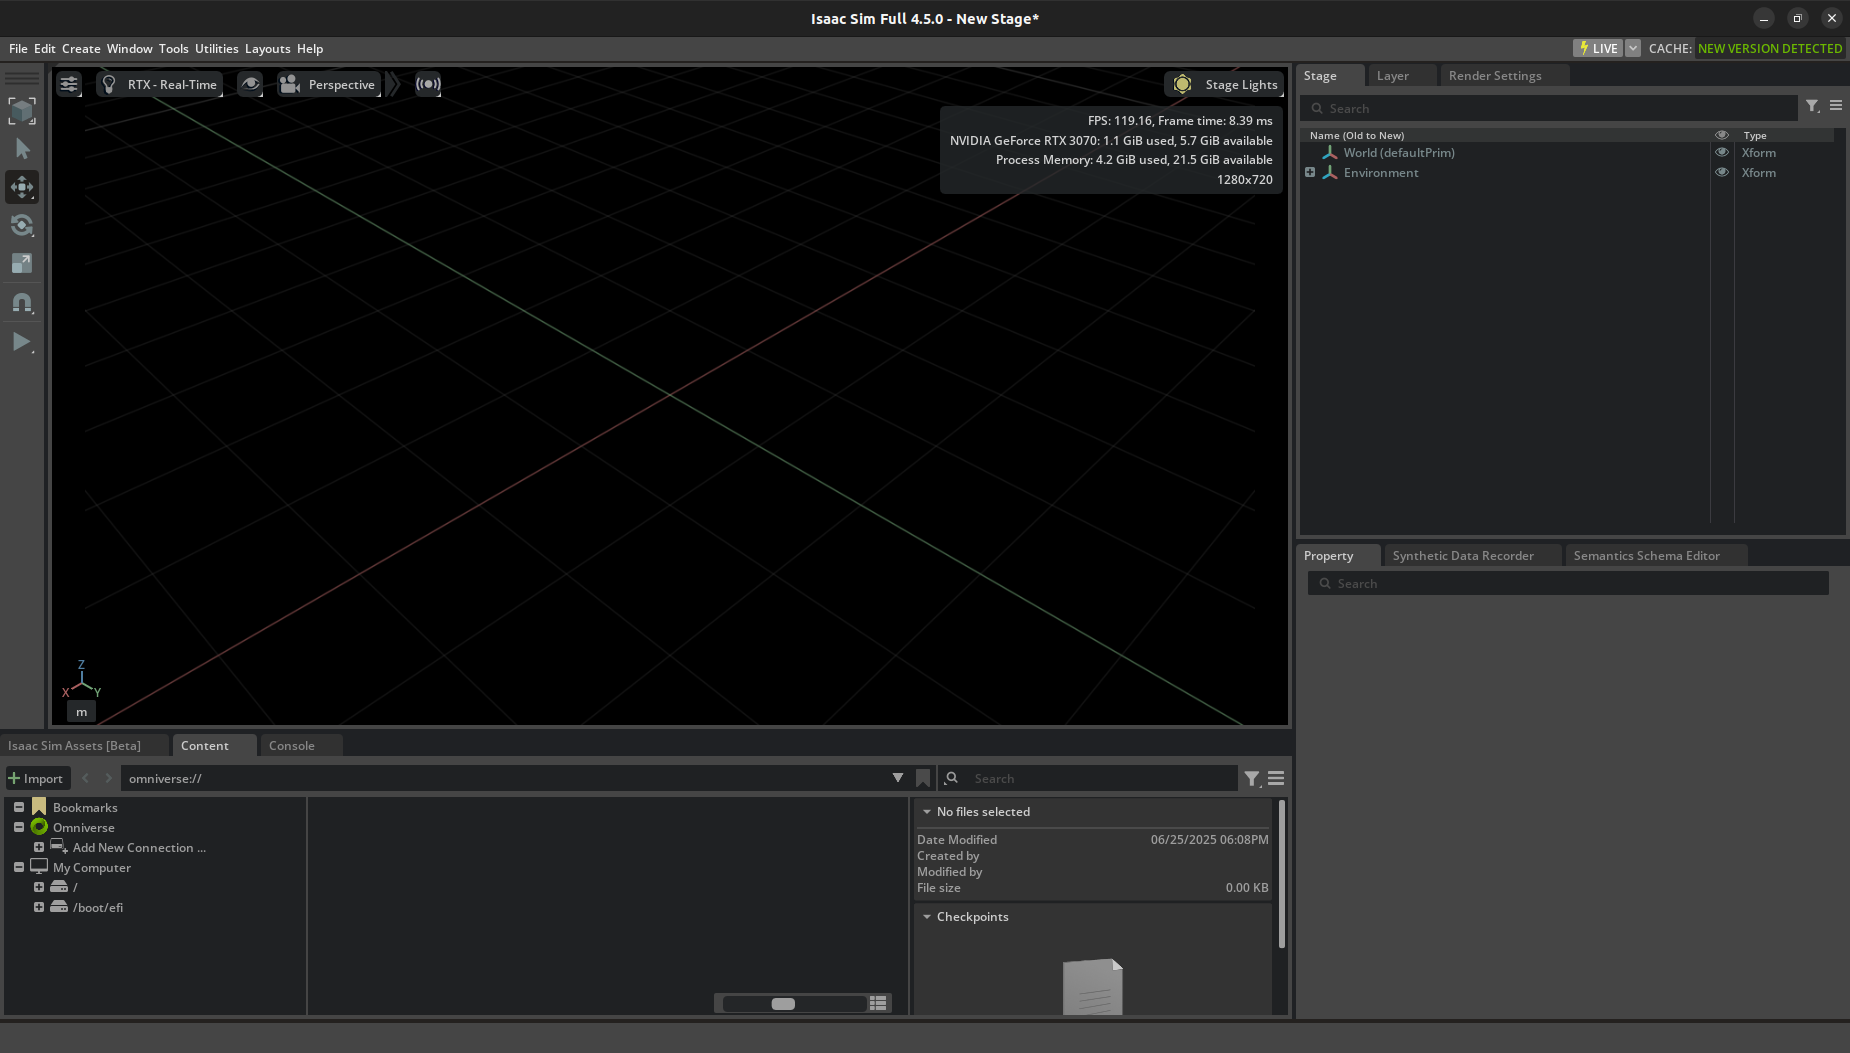
\includegraphics[width=0.75\linewidth]{Zdjęcia/widokISAACSIM.png}
    \caption{Środowisko ISAAC SIM 4.5.0}
    \label{srodowiskoISAACSIM}
\end{figure}

\clearpage

\subsection{Jak można sterować symulowanym obiektem?}

\noindent Sterowanie symulowanym obiektem w ramach programów komputerowych, takich jak symulatory fizyki czy cyfrowe bliźniaki, polega na wykorzystywaniu różnych interfejsów i narzędzi dostępnych w oprogramowaniu, które umożliwiają manipulowanie wirtualnymi obiektami. Programy takie oferują różne metody sterowania, które pozwalają na interakcję z wirtualnym modelem obiektu lub systemu. \\

\begin{enumerate}
    \item \textbf{Interfejsy graficzne (GUI)} \\
    Większość symulatorów fizyki i cyfrowych bliźniaków oferuje interfejsy graficzne, które pozwalają użytkownikowi na bezpośrednią manipulację obiektami w wirtualnym środowisku. W takich programach można:
    \begin{itemize}
        \item kliknąć i przeciągać obiekty w celu ich przesunięcia, obrotu lub zmiany parametrów (np. położenie, prędkość, kąt),
        \item używać suwaków i pól tekstowych do ustawiania parametrów takich jak masa, siła, temperatura,
        \item wizualizować obiekty w trójwymiarze i kontrolować ich orientację oraz interakcje.
    \end{itemize}
    
    \item \textbf{Sterowanie za pomocą języków programowania} \\
    Wiele symulatorów umożliwia sterowanie obiektami poprzez skrypty i programowanie w językach takich jak Python, C++, MATLAB czy dedykowane języki skryptowe:
    \begin{itemize}
        \item tworzenie skryptów sterujących ruchem i zachowaniem obiektów (np. sterowanie robotami),
        \item implementacja funkcji reagujących na zmiany warunków (np. nowe trajektorie, zmiana prędkości),
        \item integracja z zewnętrznymi systemami (czujniki, bazy danych) w czasie rzeczywistym.
    \end{itemize}
    
    \item \textbf{Zdalne sterowanie (Remote Control)} \\
    Zaawansowane systemy umożliwiają zdalne sterowanie obiektami:
    \begin{itemize}
        \item przesyłanie komend do wirtualnych obiektów przez interfejsy API lub systemy komunikacyjne,
        \item kontrolowanie obiektów w czasie rzeczywistym za pomocą komputera, aplikacji mobilnych lub kontrolerów (joysticki, pady).
    \end{itemize}
    
    \item \textbf{Sterowanie przy pomocy algorytmów sztucznej inteligencji (AI)} \\
    Symulatory wykorzystują algorytmy AI do autonomicznego sterowania obiektami:
    \begin{itemize}
        \item zastosowanie uczenia maszynowego (np. uczenie poruszania się po trudnym terenie),
        \item implementacja algorytmów sterowania (np. DQN -- Deep Q-Network), które optymalizują działania obiektów na podstawie nagród i kar.
    \end{itemize}
    
    \item \textbf{Sterowanie za pomocą interfejsów fizycznych} \\
    Niektóre symulatory pozwalają na sterowanie za pomocą urządzeń fizycznych:
    \begin{itemize}
        \item joysticki i pady do sterowania robotami, pojazdami itp.,
        \item urządzenia VR umożliwiające kontrolę w przestrzeni 3D,
        \item systemy hapticzne (np. rękawice) pozwalające na odczuwanie dotyku i oporu w interakcji z obiektami.
    \end{itemize}
    
    \item \textbf{Symulacja w oparciu o dane sensoryczne} \\
    Sterowanie obiektami może również odbywać się na podstawie danych z czujników:
    \begin{itemize}
        \item reakcje na dane sensoryczne (np. obrazy z kamer, dane z lidarów),
        \item algorytmy analizy danych w czasie rzeczywistym do modyfikacji parametrów i trajektorii.
    \end{itemize}
\end{enumerate}

Przykłady popularnych programów do sterowania symulowanymi obiektami:

\begin{itemize}
    \item \textbf{ROS (Robot Operating System)} – Oprogramowanie open-source wykorzystywane w robotyce, które umożliwia sterowanie robotami w symulacjach oraz w rzeczywistym świecie. ROS umożliwia interakcję z robotami poprzez interfejsy API oraz programowanie sterowania.
    
    \item \textbf{Gazebo} – Platforma symulacyjna dla robotów, która integruje się z ROS, oferując realistyczne środowisko do testowania robotów i innych obiektów.
    
    \item \textbf{Unity3D} – Popularna platforma do tworzenia gier, ale również wykorzystywana do symulacji obiektów 3D. Można w niej tworzyć realistyczne środowiska i sterować obiektami poprzez programowanie lub interfejsy GUI.
    
    \item \textbf{MATLAB/Simulink} – Umożliwia modelowanie i sterowanie systemami inżynierskimi, symulowanie ruchów maszyn, robotów, a także procesów przemysłowych.
\end{itemize}

\subsection{Środowisko ROS2}

ROS2 (Robot Operating System 2) to nowoczesna, otwartoźródłowa platforma operacyjna zaprojektowana z myślą o robotach nowej generacji. Jest to ewolucja klasycznego ROS1, który stał się fundamentem dla wielu projektów robotycznych na całym świecie. ROS 2 jest dedykowany do budowy bardziej złożonych i~ skalowalnych systemów robotycznych, które wymagają elastyczności, rozproszonego przetwarzania i zaawansowanego sterowania. Dzięki ROS2, twórcy systemów robotycznych mogą projektować aplikacje oparte na modularnej architekturze, gdzie poszczególne komponenty (węzły) komunikują się ze sobą, wymieniając dane przez tematy (topics), usługi (services) i akcje (actions).\\

\noindent Kluczowe cechy ROS~2:

\begin{itemize}
    \item \textbf{Modularna architektura:} ROS2 wykorzystuje koncepcję węzłów (nodes), które pełnią rolę oddzielnych, niezależnych modułów systemu. Każdy węzeł odpowiada za określoną funkcjonalność, jak na przykład sterowanie robotem, przetwarzanie danych z czujników, komunikacja z innymi urządzeniami itp. Węzły mogą się komunikować za pomocą różnych mechanizmów, takich jak tematy, usługi i akcje. Takie podejście umożliwia elastyczne projektowanie systemów robotycznych i łatwą integrację z różnymi technologiami.
    
    \item \textbf{DDS jako warstwa komunikacyjna:} Jedną z najistotniejszych zmian w ROS2 względem ROS1 jest zastosowanie standardu DDS (Data Distribution Service) jako warstwy komunikacyjnej. DDS zapewnia deterministyczne i wydajne przesyłanie danych między węzłami, zarówno w systemach lokalnych, jak i~ rozproszonych. Dzięki DDS możliwe jest przesyłanie danych w czasie rzeczywistym, co jest niezbędne w~ przypadku systemów robotycznych, które muszą reagować na zmiany w otoczeniu w czasie rzeczywistym. DDS wspiera różne polityki QoS (Quality of Service), co pozwala na dostosowanie komunikacji do wymagań systemu.
    
    \item \textbf{Wsparcie dla różnych języków programowania:} ROS2 wspiera kilka języków programowania, w~ tym C++ i Python, które są najczęściej wykorzystywane w robotyce. Dzięki temu programiści mogą wybierać odpowiedni język do realizacji poszczególnych zadań. C++ jest preferowane do aplikacji wymagających wysokiej wydajności, natomiast Python jest często używany do prototypowania i pracy z algorytmami AI/ML.
    
    \item \textbf{Interoperacyjność z popularnymi narzędziami robotycznymi i symulatorami:} ROS2 jest kompatybilny z wieloma popularnymi narzędziami wykorzystywanymi w robotyce, co czyni go bardzo wszechstronnym środowiskiem. Na przykład, ROS2 współpracuje z symulatorami takimi jak Gazebo, Isaac Sim czy Webots, które pozwalają na testowanie robotów w wirtualnym środowisku przed ich wdrożeniem w rzeczywistości. Współpracuje także z narzędziami do planowania ruchu i manipulacji, takimi jak MoveIt~2, co umożliwia kompleksowe projektowanie i testowanie aplikacji robotycznych.
    
    \item \textbf{Zastosowanie w różnych branżach robotyki:} ROS2 znajduje zastosowanie w szerokim zakresie dziedzin robotyki, w tym w robotyce przemysłowej, mobilnej, medycznej i badawczej. W robotyce przemysłowej ROS2 jest wykorzystywany do automatyzacji procesów produkcyjnych, w robotyce mobilnej – do tworzenia autonomicznych pojazdów i robotów mobilnych, a w robotyce medycznej – do wspomagania rehabilitacji i przeprowadzania skomplikowanych zabiegów. Ponadto, dzięki dużej elastyczności, ROS2 jest używany także w projektach badawczo-rozwojowych.
    
    \item \textbf{Rozproszone systemy i skalowalność:} ROS2 wspiera rozproszone systemy robotyczne, co oznacza, że węzły mogą być uruchamiane na różnych komputerach lub urządzeniach, a ich komunikacja odbywa się przez sieć. Dzięki tej funkcjonalności, ROS2 jest odpowiedni do projektów, które wymagają dużej skalowalności, takich jak systemy robotów pracujących w złożonych środowiskach, np. w magazynach, fabrykach czy w przestrzeniach miejskich.
    
    \item \textbf{Real-time capabilities:} ROS2 oferuje możliwości obsługi systemów czasu rzeczywistego, co jest istotne w przypadku aplikacji, które wymagają szybkich reakcji na zmiany w otoczeniu, jak na przykład roboty mobilne, systemy autonomiczne czy roboty współpracujące (coboty). Dzięki mechanizmom DDS i wsparciu dla systemów czasu rzeczywistego, ROS2 umożliwia wykonywanie zadań z deterministycznymi opóźnieniami.
    
    \item \textbf{Obsługa różnych platform:} ROS2 jest zaprojektowane z myślą o pracy na różnych platformach sprzętowych, w tym na komputerach PC, urządzeniach mobilnych, a także na specjalistycznych systemach wbudowanych. ROS2 wspiera systemy operacyjne takie jak Linux, Windows oraz macOS, co pozwala na jego szerokie zastosowanie w różnych środowiskach.\\
\end{itemize}

\noindent ROS2 to potężne narzędzie, które rewolucjonizuje sposób, w jaki projektowane i realizowane są systemy robotyczne. Dzięki zastosowaniu nowoczesnych technologii, takich jak DDS, wsparciu dla wielu języków programowania, narzędzi robotycznych i symulatorów, ROS2 umożliwia tworzenie skalowalnych, elastycznych i zaawansowanych systemów robotycznych. Jego wszechstronność sprawia, że znajduje zastosowanie w~ różnych dziedzinach robotyki, od przemysłu po medycynę, a także w badaniach naukowych, gdzie precyzyjne sterowanie i szybkie reakcje na zmiany w otoczeniu są kluczowe.

\subsection{Czym jest robot mobilny?}

Robot mobilny to autonomiczne lub zdalnie sterowane urządzenie, które posiada zdolność przemieszczania się w przestrzeni. W odróżnieniu od robotów stacjonarnych (np. ramion robotycznych), roboty mobilne mogą zmieniać swoje położenie względem otoczenia, co pozwala im na realizację zadań takich jak eksploracja, transport, inspekcja czy wsparcie operacyjne w środowiskach dynamicznych. Ruch robota może być realizowany na różne sposoby – za pomocą kół, gąsienic, nóg lub kombinacji tych elementów. Roboty mobilne są szeroko wykorzystywane zarówno w przemyśle, jak i w zastosowaniach cywilnych oraz wojskowych, a rozwój technologii czujników, algorytmów sterowania i sztucznej inteligencji umożliwia im coraz bardziej samodzielne funkcjonowanie w złożonych środowiskach.


\subsection{Typy robotów mobilnych}

\noindent Roboty mobilne można podzielić na różne typy w zależności od sposobu ich poruszania się. Najpopularniejsze z nich to roboty kołowe oraz roboty kroczące.\\

\noindent Roboty kołowe wykorzystują koła jako podstawowy mechanizm napędu i kierowania. Tego typu konstrukcje są technicznie prostsze, bardziej energooszczędne i łatwiejsze w sterowaniu, zwłaszcza na płaskich, utwardzonych powierzchniach. Dzięki prostemu modelowi kinematycznemu, sterowanie ruchem takiego robota (np. skręcanie, jazda po łuku) można łatwo realizować za pomocą stosunkowo nieskomplikowanych algorytmów. Z tego względu roboty kołowe są często stosowane w robotyce edukacyjnej, magazynowej czy inspekcyjnej.\\

\noindent Roboty kroczące typu quadruped, czyli roboty czworonożne, są znacznie bardziej zaawansowane pod względem konstrukcyjnym i sterowania. Poruszają się w sposób zbliżony do zwierząt, co pozwala im na pokonywanie trudnych, nieregularnych terenów, gdzie roboty kołowe nie mogłyby się poruszać. Jednak taka forma lokomocji wymaga złożonych algorytmów równoważenia, planowania kroków i stabilizacji postawy, co czyni sterowanie nimi znacznie trudniejszym. Pomimo tej złożoności, roboty quadruped zyskują na popularności w~ zastosowaniach terenowych, ratowniczych i wojskowych ze względu na swoją mobilność i adaptacyjność.

\subsection{Unitree Go2 EDU}

\noindent Unitree Go2 EDU to zaawansowany robot mobilny o czterokończynowej konstrukcji, zaprojektowany przez firmę Unitree Robotics – jednego z liderów w dziedzinie robotyki kroczącej. Model ten stanowi wersję edukacyjną (EDU), oferując rozszerzone możliwości programistyczne i integracyjne względem wersji konsumenckiej. Dzięki otwartemu środowisku programowania, rozbudowanemu układowi sensorycznemu oraz dużej mobilności, znajduje zastosowanie w edukacji wyższej, pracach badawczo-rozwojowych, a także w zadaniach inspekcyjnych i eksperymentalnych.\\

\noindent Korpus robota wykonano z lekkich i wytrzymałych materiałów – głównie stopów aluminium i włókien węglowych. Robot porusza się na czterech kończynach o trzech stopniach swobody każda (12 DOF), napędzanych przez wydajne, bezszczotkowe silniki z czujnikami momentu. Taka konfiguracja zapewnia płynny, dynamiczny chód z możliwością dostosowania kroku do zmiennych warunków terenowych, a także wykonywanie złożonych manewrów, takich jak omijanie przeszkód, wchodzenie po schodach czy skoki.\\

\noindent W wersji EDU robot wyposażony jest w szereg czujników, umożliwiających percepcję otoczenia i autonomiczne działanie. W skład systemu sensorycznego wchodzą:
\begin{itemize}
    \item Kamera głębokości (np. Intel RealSense)
    \item 9-osiowy IMU (żyroskop + akcelerometr + magnetometr)
    \item Enkodery położenia i momentu
    \item LIDAR 2D/3D (opcjonalnie)
    \item Mikrofony i czujniki dźwięku
    \item Opcjonalna kamera RGB i termowizyjna
\end{itemize}

\noindent Sercem systemu sterowania jest minikomputer klasy NVIDIA Jetson Orin lub komputer przemysłowy z~ systemem Linux Ubuntu, z preinstalowanym środowiskiem ROS 2 (Robot Operating System). Umożliwia to rozwój własnych algorytmów z zakresu SLAM, autonomicznej nawigacji, rozpoznawania obiektów, oraz komunikacji człowiek–robot.\\


\noindent Robot może być sterowany na trzy sposoby:
\begin{itemize}
    \item Zdalnie, za pomocą dedykowanego kontrolera lub aplikacji mobilnej.
    \item Z poziomu komputera, przez połączenie Wi-Fi, Bluetooth lub Ethernet.
    \item Autonomicznie, poprzez zaprogramowane algorytmy w ROS 2.
\end{itemize}
Do dyspozycji użytkownika oddano interfejsy API w językach Python i C++, umożliwiające pełne sterowanie ruchem, przetwarzaniem danych z czujników i integracją z dodatkowymi modułami.\\

\noindent Unitree Go2 EDU znajduje zastosowanie w szerokim zakresie dziedzin technicznych i naukowych, w tym:
\begin{itemize}
    \item Robotyka mobilna i biomechanika – modelowanie ruchu, optymalizacja lokomocji, analiza chodu
    \item Nawigacja autonomiczna i SLAM – mapowanie środowiska i eksploracja przestrzeni
    \item Widzenie maszynowe i sztuczna inteligencja – rozpoznawanie gestów, twarzy, przeszkód
    \item Przemysł i inspekcja – patrolowanie zakładów przemysłowych, kontrola infrastruktury technicznej
    \item Działania ratunkowe i wojskowe – misje w środowiskach nieprzyjaznych człowiekowi (gruzowiska, strefy skażone)
    \item Edukacja i dydaktyka – nauczanie sterowania, analizy danych sensorycznych, projektowania systemów embedded
\end{itemize}


Specyfikacja techniczna:
\begin{itemize}
    \item \textbf{Wymiary (wysokość x szerokość x długość)}: 70x31x40 cm (pozycja stojąca), 76x31x20 cm (pozycja kucająca)
    \item \textbf{Waga (z baterią)}: Około 15 kg
    \item \textbf{Materiał}: Stop aluminium + wysoka wytrzymałość plastiku inżynierskiego
    \item \textbf{Napięcie robocze}: 28V$ \sim$ 33.6V
    \item \textbf{Moc szczytowa}: Około 3000W
    \item \textbf{Udźwig}: Około 8 kg (maks. 12 kg)
    \item \textbf{Prędkość}: 0 $\sim$ 3.7 m/s (maks. 5 m/s)
    \item \textbf{Maksymalna wysokość podjazdu}: Około 16 cm
    \item \textbf{Kąt wspinania}: 40°
    \item \textbf{Maksymalny moment obrotowy}: Około 45 N·m
    \item \textbf{Liczba stawów motorycznych}: 12 zestawów
    \item \textbf{Zakres ruchu}: Ciało: -48° $\sim$ 48°, Udo: -200° $\sim$ 90°, Goleni: -156° $\sim$ -48°
    \item \textbf{Bateria}: Standardowa 8000 mAh, długowieczna 15000 mAh
    \item \textbf{Czas pracy}: Około 2–4 godziny
    \item \textbf{Ładowanie}: Szybkie ładowanie (33.6V 9A)
    \item \textbf{Procesor}: Nvidia Jetson Orin (opcjonalny)
    \item \textbf{Łączność}: Wi-Fi 6 (Dual-band), Bluetooth 5.2
    \item \textbf{Bateria}: Inteligentna bateria, zabezpieczona przed przegrzaniem, przeciążeniem oraz zwarciem
    \item \textbf{Inne cechy}: Głośnik do odtwarzania muzyki
\end{itemize}


Funkcje i urządzenia robota:
\begin{itemize}
    \item Moduł śledzenia: Zdalne sterowanie lub automatyczne śledzenie obiektów
    \item Mikrofon interkomowy: Umożliwia komunikację z robotem bez ograniczeń scenariuszowych
    \item Kamery i sensory:
    \begin{itemize}
        \item Kamera przednia: Transmisja obrazu w rozdzielczości 1280x720, pole widzenia 120°, szeroki kąt widzenia
        \item LIDAR 4D L1: Skanning 360° w zakresie 90°, omijanie przeszkód z minimalnymi martwymi strefami
    \end{itemize}
    \item Motory precyzyjnych stawów: 12 silników z aluminium zapewnia mocne, precyzyjne ruchy
    \item Czujniki siły w stopach: Monitorowanie sił działających na nogi robota w czasie rzeczywistym, co pozwala na dynamiczną adaptację do terenu
    \item Przenośny pasek samonawijający: Umożliwia łatwe przenoszenie robota oraz załadunek
    \item Głośnik do odtwarzania muzyki: Odtwarzanie muzyki lub dźwięków w trakcie pracy robota
\end{itemize}


\noindent Unitree Go2 EDU to wyjątkowe narzędzie dydaktyczne i badawcze, umożliwiające eksperymentowanie z~ nowoczesnymi technikami robotyki mobilnej, widzenia komputerowego oraz sztucznej inteligencji. Dzięki swojej modułowości, wszechstronności i kompatybilności z ROS 2, robot ten jest szczególnie ceniony przez uczelnie techniczne, laboratoria R\&D oraz przemysł innowacyjny.


\begin{figure}[h]
    \centering
    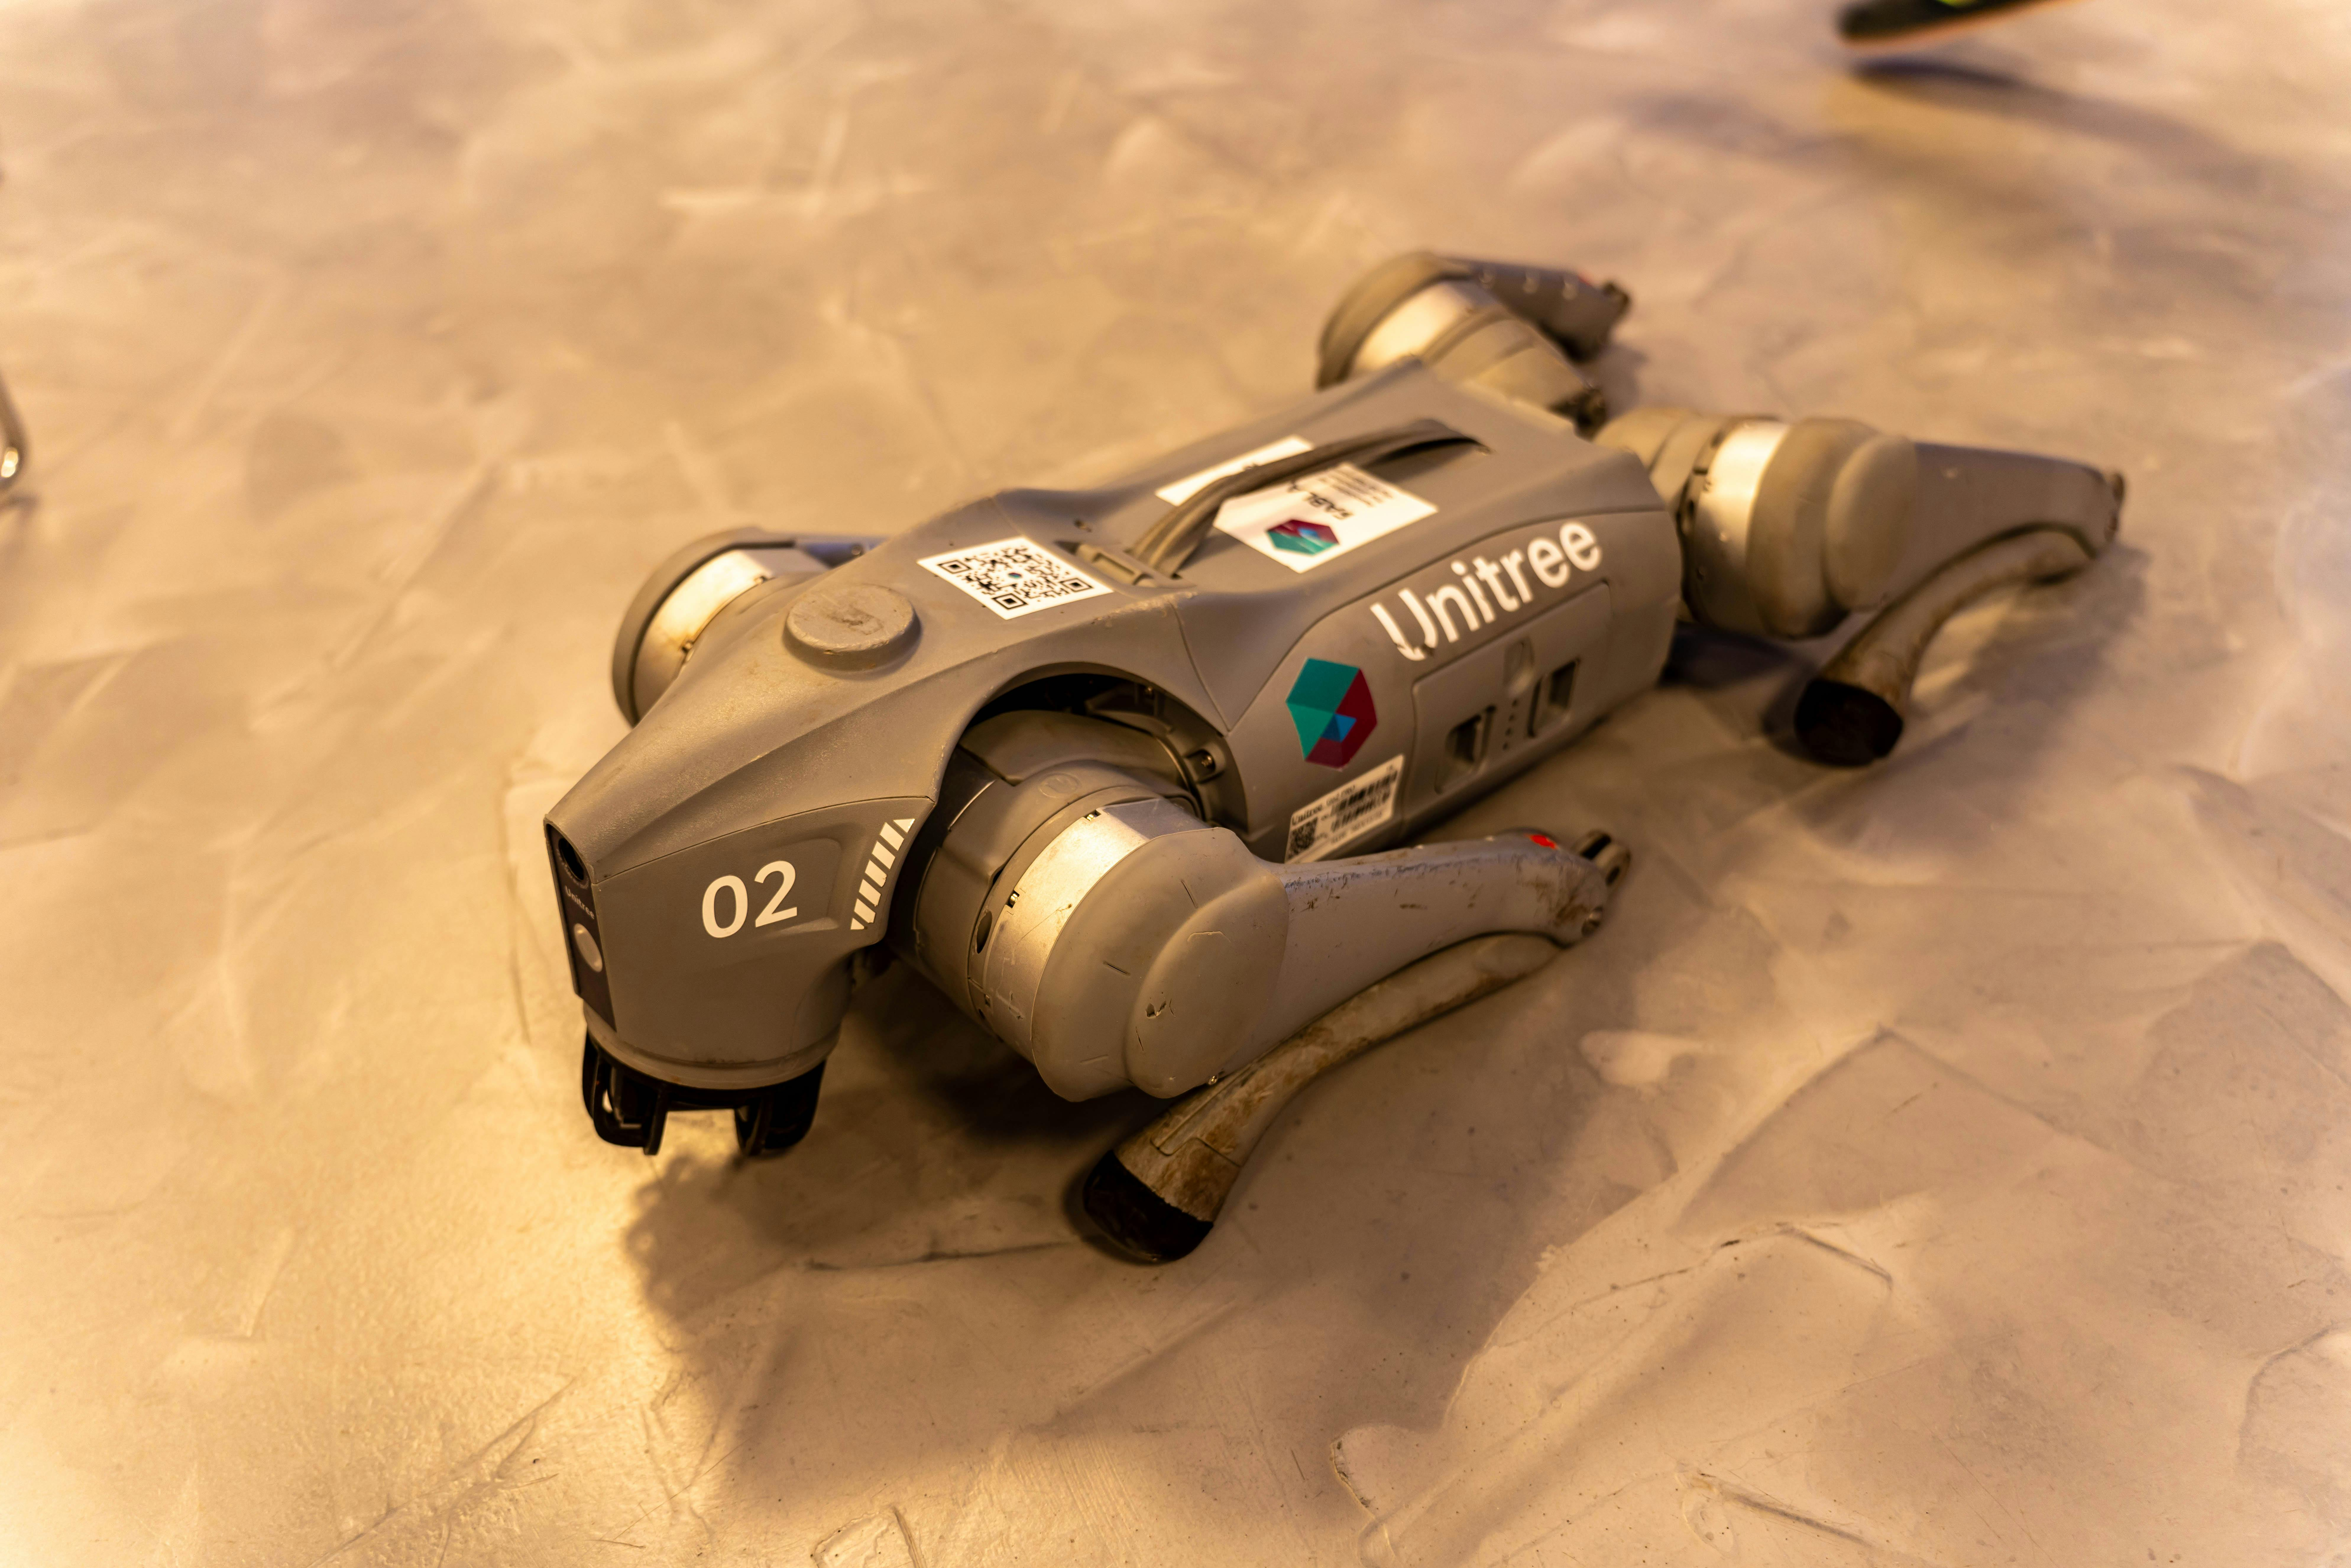
\includegraphics[width=0.75\linewidth]{Zdjęcia/prawdziwyPies.jpg}
    \caption{Robot Unitree Go2.}
    \label{prawdziwyPies}
\end{figure}

\clearpage

\section{Instalacja i konfiguracja środowiska ISSAC SIM oraz ROS2 Humble}

\subsection{Wykorzystany sprzęt}

W projekcie korzystaliśmy z systemu Ubuntu 22.04, wykorzystaliśmy system Linux ze względu na potrzebę wykorzystania środowiska ROS2 w projekcie, co jest prostsze w systemach linuxowych.\\ 

\noindent W celu realizacji projektu związanego z przygotowaniem środowiska symulacyjnego dla robota mobilnego Unitree Go2 wykorzystano dwie niezależne stacje robocze. Oba komputery zostały skonfigurowane w taki sposób, aby umożliwić pełną instalację i uruchamianie platformy Isaac Sim w wersji 4.5.0 oraz systemu ROS2 Humble, a także zapewnić odpowiednie zasoby sprzętowe do prowadzenia symulacji, testów komunikacji oraz integracji cyfrowego bliźniaka robota z oprogramowaniem.\\

\noindent Pierwsza stacja robocza była wyposażona w mobilną kartę graficzną NVIDIA GeForce RTX 3060 Laptop GPU z 6 GB pamięci VRAM, która zapewniała wymagane wsparcie dla środowiska Isaac Sim, szczególnie w zakresie renderowania 3D oraz przyspieszania obliczeń fizycznych. Sercem komputera był Intel Core i7-11800H – ośmiordzeniowy procesor z obsługą szesnastu wątków, umożliwiający płynną pracę z wieloma procesami jednocześnie. Komputer posiadał również 32 GB pamięci RAM, co pozwalało na komfortowe korzystanie z~ bibliotek ROS 2 oraz uruchamianie symulacji w czasie rzeczywistym. Dane projektowe przechowywano na szybkim dysku NVMe SSD o pojemności 512 GB, co znacznie skracało czas ładowania scen, uruchamiania narzędzi i kompilacji pakietów.\\

\noindent Druga stacja robocza, również pracująca pod kontrolą Ubuntu 22.04 LTS, była wyposażona w kartę graficzną NVIDIA GeForce RTX 3070 z 8 GB pamięci VRAM, co dawało nieco większe możliwości graficzne, szczególnie przy bardziej złożonych środowiskach symulacyjnych. W jednostce zastosowano sześciordzeniowy procesor AMD Ryzen 5 5600, który zapewniał wysoką wydajność w zastosowaniach inżynierskich i deweloperskich. Komputer ten, podobnie jak pierwszy, posiadał 32 GB pamięci RAM oraz dysk SSD o pojemności 512 GB, umożliwiający sprawną pracę z wymagającym oprogramowaniem oraz dużymi plikami danych. \\

\noindent Na obu komputerach przeprowadzono analogiczne działania, obejmujące instalację niezbędnych bibliotek systemowych, konfigurację środowiska Python, narzędzi ROS 2 oraz komponentów Isaac Sim, takich jak ros\_bridge czy dedykowane wtyczki. Stacje umożliwiały pełną pracę z cyfrowym bliźniakiem robota, jego uruchamianie w symulowanym środowisku oraz testowanie komunikacji z ROS 2. Dzięki zastosowaniu dwóch niezależnych maszyn możliwe było równoległe prowadzenie prac, co znacząco przyspieszyło postęp całego projektu.\\

\noindent Pod względem sprzętowym obie stacje spełniały wymagania środowiska Isaac Sim, w tym wymogi dotyczące akceleracji GPU oraz obsługi zaawansowanych funkcji graficznych.

\clearpage

\subsection{Test możliwości sprzętowych i systemowych}

W oprogramowaniu NVIDI dostępna jest specjalna aplikacji, pozwalająca na sprawdzenie, czy komputer z~ którego korzystamy, spełnia wymagania dla oprogramowania ISAAC SIM. Na rysunku \ref{sprzetSprawdz} pokazany jest wynik sprawdzenia jednego z wykorzystanych w projekcie komputerów.

\begin{figure}[h]
    \centering
    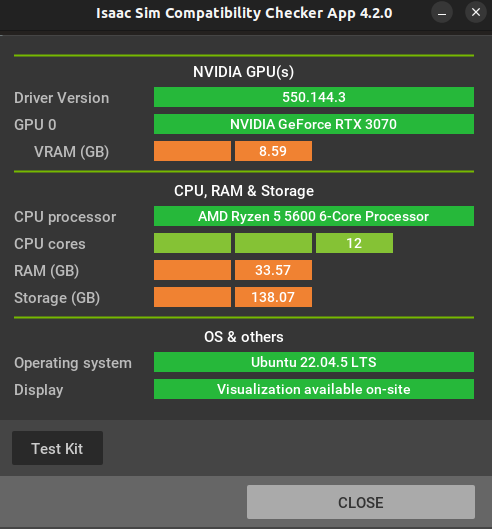
\includegraphics[width=0.5\linewidth]{Zdjęcia/sprawdzeniSprzetu.png}
    \caption{Wynik sprawdzenia kompatybilności sprzętu z ISAAC SIM.}
    \label{sprzetSprawdz}
\end{figure}

\subsection{Instalacja środowiska ISAAC SIM}

Ponieważ nie da się już pobrać ISAAC SIM bezpośrednio przy użyciu Omniverse Launcher, pobraliśmy ręcznie archiwum ze strony NVIDIA:

\begin{itemize}
    \item Strona: https://developer.nvidia.com/isaac-sim
    \item Wersja: Isaac Sim 4.5.0
\end{itemize}

\noindent Po pobraniu rozpakowaliśmy plik i możliwe było już uruchomienie środowiska ISAAC SIM. Można to zrobić, wchodząc do katalogu, w którym umieszczone zostały rozpakowane pliki i wpisując ./isaac-sim.sh lub alternatywnie isaac-sim.selector.sh.

 

\subsection{Instalacja środowiska ROS2}

Źródłem wykonanej instalacji była oficjalna dokumentacja ROS 2 dla wersji Humble (Ubuntu Development Setup):

 https://docs.ros.org/en/humble/Installation/Alternatives/Ubuntu-Development-Setup.html


\subsubsection{Krok 1: Konfiguracja lokalizacji UTF-8}
Na początku upewniliśmy się, że system ma skonfigurowane środowisko lokalizacyjne obsługujące UTF-8.


\texttt{sudo locale-gen en\_US en\_US.UTF-8}

\texttt{sudo update-locale LC\_ALL=en\_US.UTF-8 LANG=en\_US.UTF-8}

\texttt{export LANG=en\_US.UTF-8}

\noindent Sprawdziliśmy, czy ustawienia lokalne są prawidłowe:

\texttt{locale}

\subsubsection{Krok 2: Instalacja zależności systemowych}
Zainstalowaliśmy wymagane pakiety narzędziowe i kompilacyjne:

\texttt{sudo apt update \&\& sudo apt install -y}


\texttt{build-essential cmake git wget curl}


\texttt{gnupg lsb-release python3-colcon-common-extensions}


\texttt{python3-pip python3-vcstool python3-rosdep}
\\

\noindent Zainicjowaliśmy narzędzie rosdep:

\texttt{sudo rosdep init}


\texttt{rosdep update}


\subsubsection{Krok 3: Utworzenie przestrzeni roboczej i pobranie kodu ROS 2}

Stworzyliśmy katalog roboczy i pobraliśmy plik repozytoriów:


\texttt{mkdir -p $\sim$/ros2\_humble/src}

\texttt{cd $\sim$/ros2\_humble}

\texttt{wget https://raw.githubusercontent.com/ros2/ros2/humble/ros2.repos}

\texttt{vcs import src < ros2.repos}

\subsubsection{Krok 4: Instalacja zależności pakietów ROS 2}

Zainstalowaliśmy wszystkie zależności wymagane do kompilacji (pomijając rti-connext, którego nie potrzebujemy).


\texttt{rosdep install --from-paths src --ignore-src -r -y}

\texttt{--skip-keys "fastcdr rti-connext-dds-6.0.1 urdfdom\_headers}


\subsubsection{Krok 5: Kompilacja ROS 2}

Rozpoczęliśmy kompilację całego środowiska z wykorzystaniem colcon:

\texttt{cd $\sim$/ros2\_humble}

\texttt{colcon build --symlink-install}

\noindent Ten proces trwał kilkanaście minut.


\subsubsection{Krok 6: Konfiguracja środowiska}

Po zakończeniu kompilacji dodaliśmy ROS 2 do zmiennych środowiskowych:

\texttt{echo "source $\sim$/ros2\_humble/install/setup.bash" $>>$ $\sim$/.bashrc}

\texttt{source $\sim$/.bashrc}

\noindent Dzięki temu komenda ros2 była dostępna z każdego terminala.

\subsubsection{Weryfikacja działania ROS2 }

Przeprowadziliśmy podstawowy test komunikacji między dwoma węzłami:

Terminal 1:

\texttt{ros2 run demo\_nodes\_cpp talker}


Terminal 2:

\texttt{ros2 run demo\_nodes\_cpp listener}
\\
Terminal listener poprawnie odbierał wiadomości wysyłane przez talker, co potwierdziło, że środowisko działa.



\section{Jazda robotem kołowym z użyciem ROS2 i teleop\_twist\_keyboard}

\noindent Pakiet teleop\_twist\_keyboard umożliwia ręczne sterowanie robotem mobilnym w systemie ROS2 z użyciem klawiatury. Wysyła komunikaty typu geometry\_msgs/msg/Twist na zadany temat (domyślnie /cmd\_vel). Pozwala sterować prędkością liniową oraz kątową - co jest typowym sposobem poruszania się robotów mobilnych (np. typu differential drive).\\

\noindent Podstawowe sterowanie odbywa się z użyciem następujących klawiszy:\\

\texttt{i  Do przodu}

\texttt{k  Zatrzymanie(zerowanie prędkości)}

\texttt{,  Do tyłu}

\texttt{j  Skręt w lewo(obrót w miejscu)}

\texttt{l  Skręt w prawo(obrót w miejscu)}

\texttt{u Do przodu + w lewo}

\texttt{o  Do przodu + w prawo}

\texttt{m  Do tyłu + w lewo}

\texttt{.  Do tyłu + w prawo}\\
 
\noindent Zmiana prędkości:\\

\texttt{q  Zwiększ prędkość liniową i kątową}

\texttt{z  Zmniejsz prędkość liniową i kątową}

\texttt{w  Zwiększ tylko prędkość liniową}

\texttt{x  Zmniejsz tylko prędkość liniową}

\texttt{e  Zwiększ tylko prędkość kątową}

\texttt{c  Zmniejsz tylko prędkość kątową}\\

\noindent Każde wciśnięcie odpowiedniego klawisza powoduje wysłanie wiadomości Twist na zadany temat, zgodnie z~ bieżącymi wartościami prędkości.\\

\noindent Instalacja pakietu

\texttt{a) instalacja binarna zalecana}

\texttt{sudo apt update}

\texttt{sudo apt install ros-humble-teleop-twist-keyboard}

\texttt{b) Instalacja ze źródła}

\texttt{cd $\sim$/ros2\_ws/src}

\texttt{git clone https://github.com/ros2/teleop\_twist\_keyboard.git}

\texttt{cd ..}

\texttt{colcon build}

\texttt{source install/setup.bash}

\texttt{Uruchomienie}

\texttt{ros2 run teleop\_twist\_keyboard teleop\_twist\_keyboard}\\

\noindent Do testów wykorzystano gotowy przykład robota mobilnego dostępny w środowisku Isaac Sim 4.5.0, który został przygotowany do współpracy z systemem ROS2. Przykład ten zawiera wstępnie skonfigurowany zestaw węzłów (nodes) ROS2, które umożliwiają komunikację pomiędzy symulowanym robotem, a zewnętrznym środowiskiem ROS 2. \\

\noindent Robot ten subskrybuje wiadomości typu geometry\_msgs/msg/Twist, publikowane na temacie /cmd\_vel, który jest domyślnym kanałem komunikacyjnym wykorzystywanym przez pakiet teleop\_twist\_keyboard. Oznacza to, że po uruchomieniu symulacji oraz włączeniu mostu ROS 2, komendy wysyłane z klawiatury mogą bezpośrednio sterować ruchem robota w symulacji.

\begin{figure}[h]
    \centering
    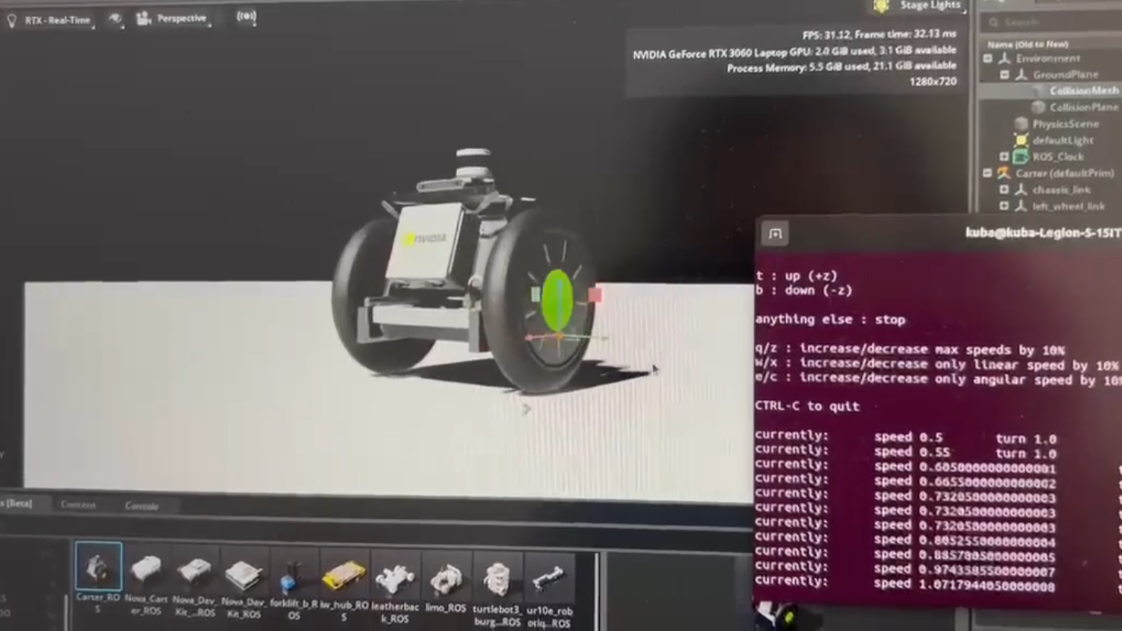
\includegraphics[width=0.8\linewidth]{Zdjęcia/robocikRos2.png}
    \caption{Robot kołowy w symulacji ISAAC SIM.}
    \label{fig:robotKolowy}
\end{figure}


\section{Cyfrowy bliźniak robota Unitree Go2}

\subsection{Podejście od strony opisywanej w dokumentacji producenta}

\noindent W pierwszej kolejności podczas realizacji projektu podjęto próbę przygotowania cyfrowego bliźniaka robota Unitree Go2 zgodnie z dokumentacją techniczną oraz materiałami udostępnianymi przez producenta. Firma Unitree oferuje oficjalny zestaw ROS2 SDK (Software Development Kit), który rzekomo umożliwia komunikację z robotem, jego sterowanie oraz wykorzystanie gotowego modelu robota do integracji w zewnętrznych środowiskach, takich jak Gazebo, RViz czy inne narzędzia wizualizacyjne kompatybilne z ROS2. Na potrzeby tej części projektu przeanalizowano zawartość dokumentacji oraz repozytoriów publicznych dostępnych za pośrednictwem platformy GitHub\\

\noindent Na oficjalnej stronie producenta oraz w dokumentacji SDK dostępnej online, wskazywane są dwa podstawowe źródła informacji:

\begin{itemize}
    \item Pakiety SDK dla fizycznego robota,
    \item Skrypty integracyjne z ROS/ROS2,
    \item Opcjonalne materiały do wykorzystania modelu w symulacji. 
\end{itemize}

\noindent W dokumentacji znajduje się ogólny opis struktury danych przesyłanych między robotem a komputerem użytkownika, formaty wiadomości, a także wskazówki dotyczące uruchamiania środowiska ROS. Szczególnie istotne były odniesienia do obsługi czujników, takich jak IMU, LiDAR oraz danych z enkoderów nóg, które mają kluczowe znaczenie w kontekście wirtualnej symulacji.\\

\begin{figure}[h]
    \centering
    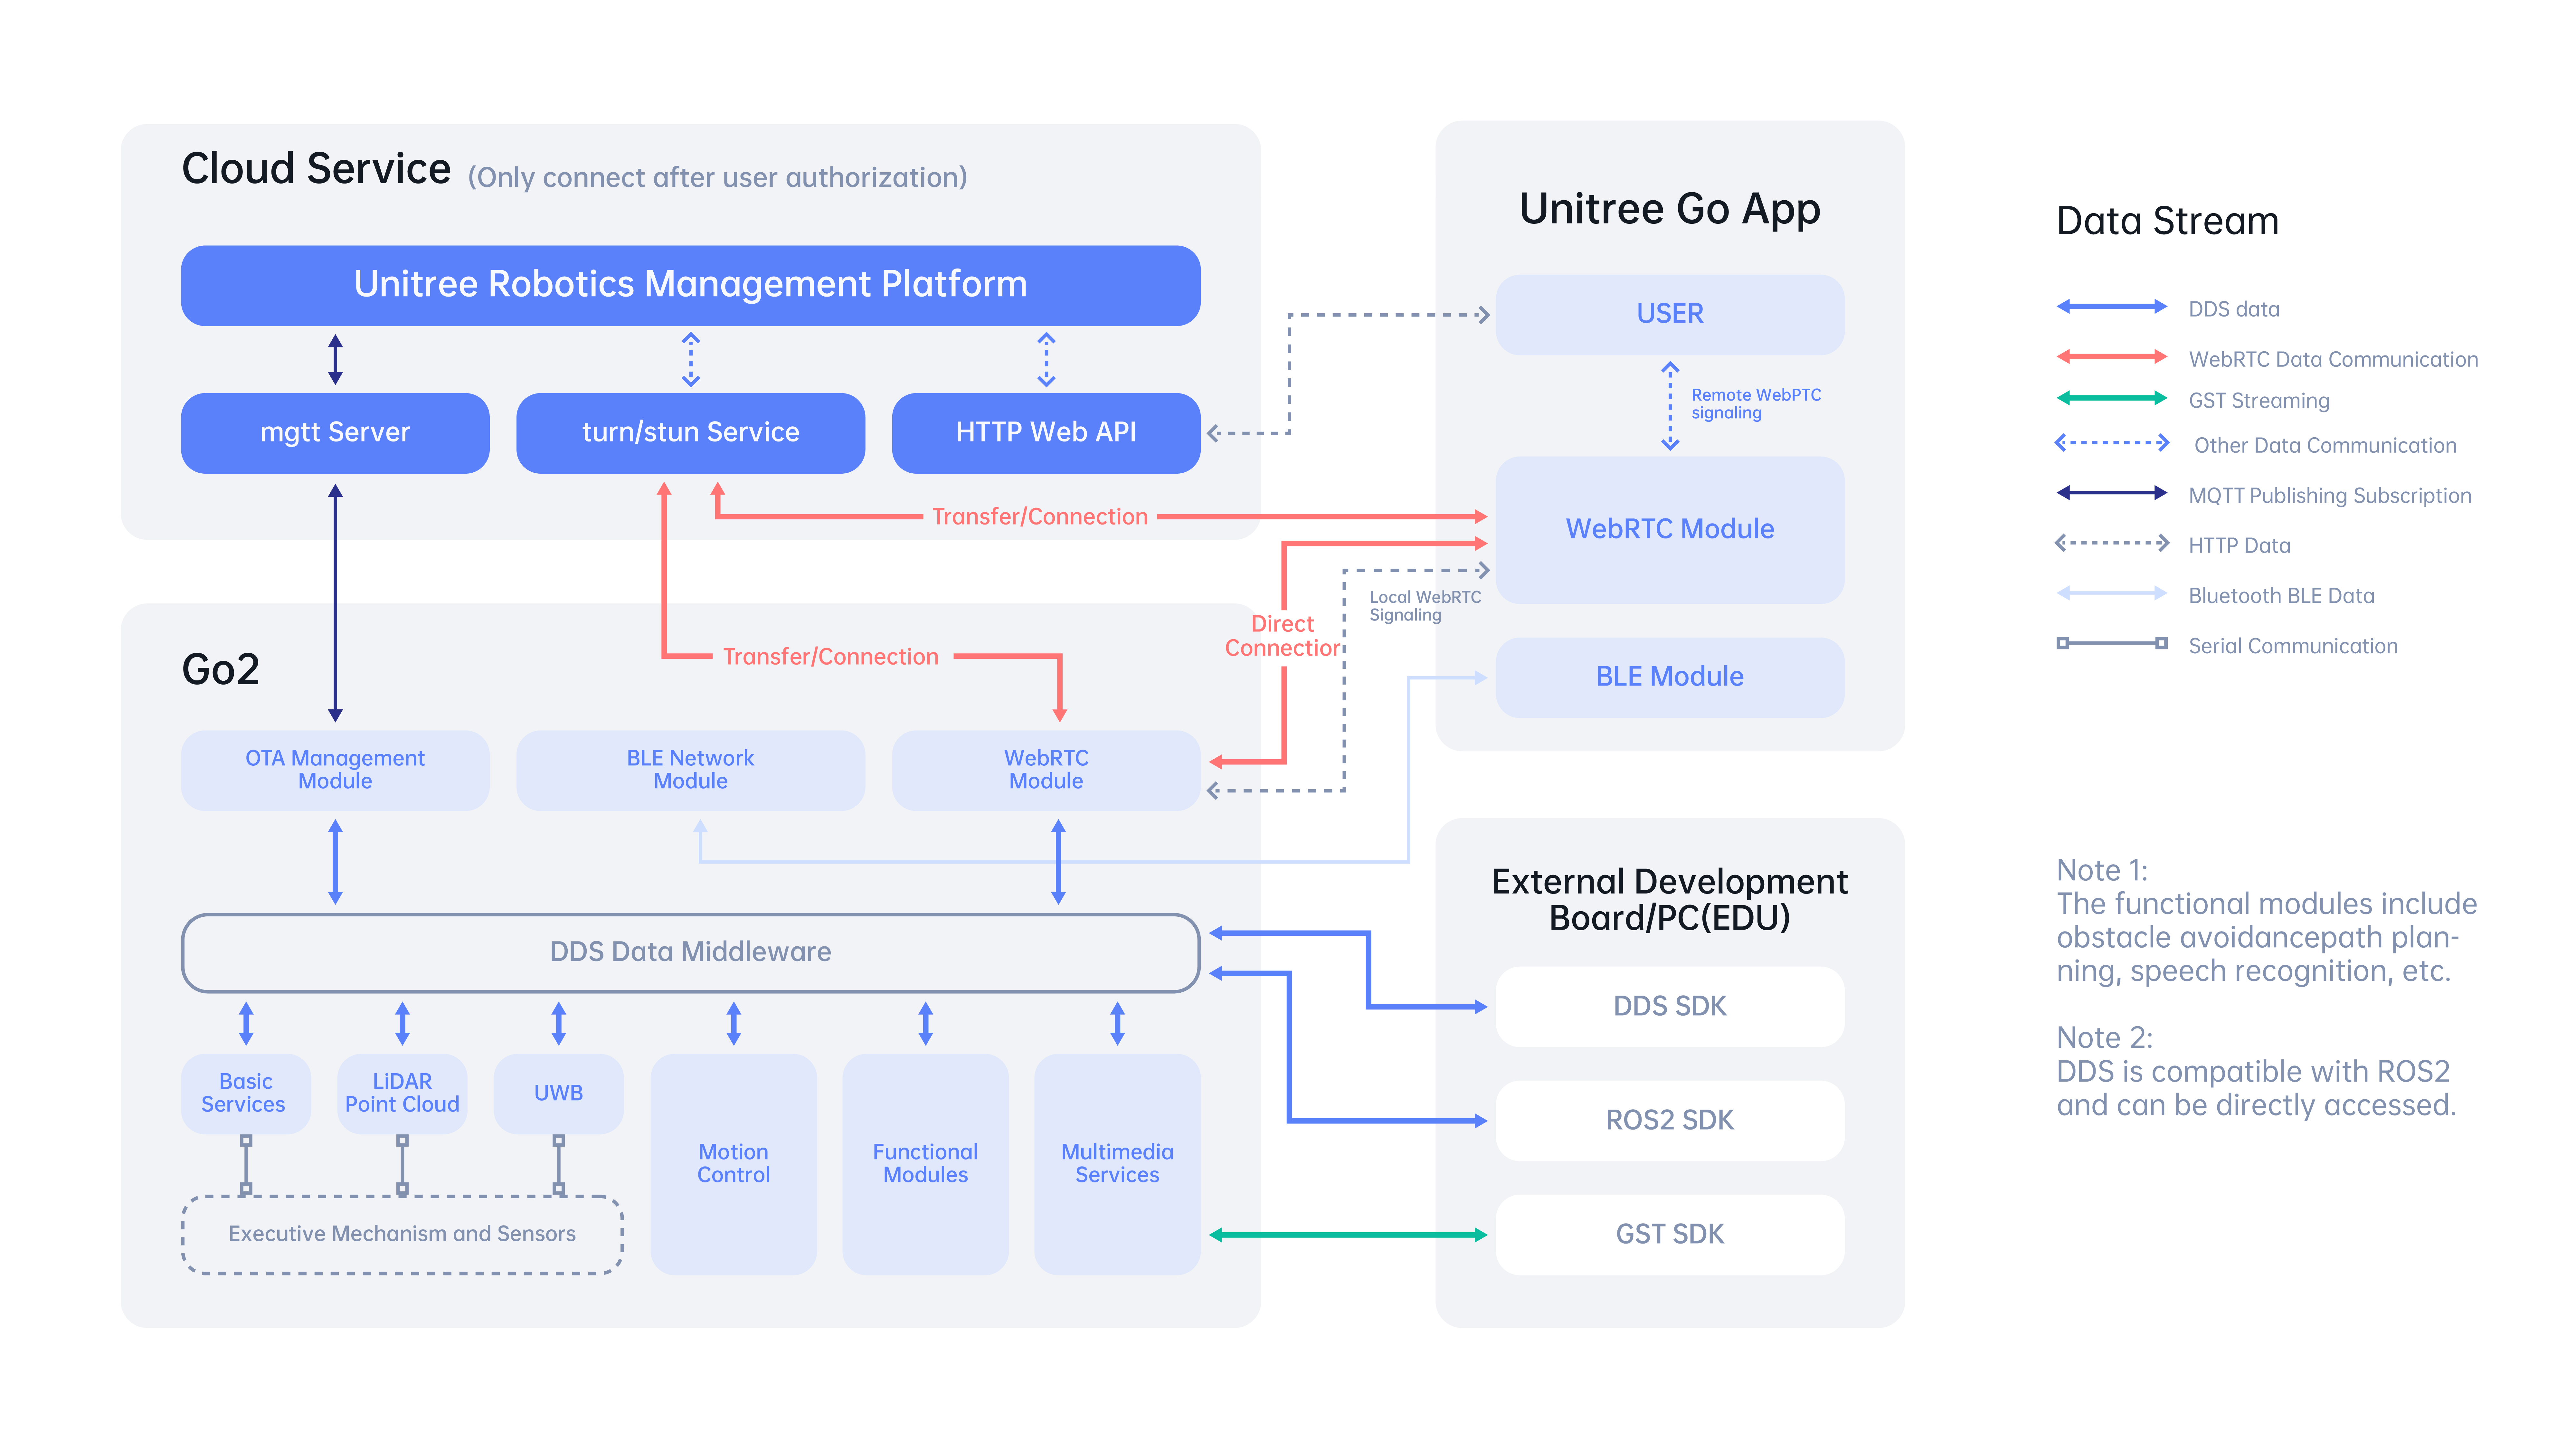
\includegraphics[width=1\linewidth]{Zdjęcia/schematKomunikacji.png}
    \caption{Schemat komunikacji robota Unitree Go2}
    \label{fig:schematKomunikacji}
\end{figure}

Zgodnie z materiałami producenta, w celu stworzenia środowiska symulacyjnego należy:
\begin{enumerate}
    \item Zainstalować ROS 2 (zalecana wersja Humble lub Foxy),
    \item Skonfigurować zależności SDK oraz skompilować pakiety za pomocą colcon build,
    \item Uruchomić symulację w środowisku Gazebo lub innym kompatybilnym,
    \item Skorzystać z udostępnionego modelu URDF lub SDF robota Go2,
    \item Uruchomić most ROS–symulator
    \item Sterować robotem z wykorzystaniem przykładowych skryptów z SDK. 
\end{enumerate}


\noindent \textbf{Praktyczna weryfikacja dokumentacji}\\

\noindent Pomimo że dokumentacja producenta wskazuje dość bezpośrednie ścieżki konfiguracji środowiska, próby praktycznego wdrożenia opisanego procesu napotkały na szereg trudności. Pierwszym i najbardziej istotnym problemem była jakość oraz kompletność udostępnionych materiałów. Już na etapie klonowania repozytoriów SDK napotkano na niespójności – niektóre pliki wymagane do kompilacji nie były dostępne publicznie, inne zawierały błędy składniowe, a część nie była zgodna z wersją ROS2 Humble.\\

\noindent W toku testów okazało się również, że sam SDK – przynajmniej w formie publicznie dostępnej – nie umożliwia uruchomienia wirtualnego modelu robota w żadnym popularnym środowisku symulacyjnym. Brakowało kompletnych opisów plików URDF/SDF, brakowało tekstur, plików konfiguracji czujników oraz definicji dynamicznych właściwości robota (np. momentów bezwładności, ograniczeń przegubów). Próba samodzielnej kompilacji i uruchomienia wskazanych przykładów kończyła się błędami już na poziomie budowy pakietów lub ich inicjalizacji.\\

\noindent Dodatkowo, znaczna część kodu źródłowego była przygotowana z myślą o bezpośrednim połączeniu z fizycznym robotem, a nie z symulacją. Oznaczało to, że próby wykorzystania tych samych skryptów do kontrolowania modelu cyfrowego kończyły się niepowodzeniem – brakowało bowiem warstwy abstrakcji pozwalającej na przełączanie między fizycznym a wirtualnym środowiskiem.\\

\noindent \textbf{Brak wsparcia dla Isaac Sim}\\

\noindent Kolejną istotną obserwacją był całkowity brak oficjalnego wsparcia dla środowiska Isaac Sim w ramach materiałów dostarczanych przez Unitree. Mimo że Isaac Sim staje się coraz popularniejszą platformą do symulacji robotów dzięki wsparciu NVIDIA, dokumentacja producenta robota Go2 nie przewiduje jego wykorzystania. Brakuje nie tylko odpowiednich rozszerzeń do formatu USD (Universal Scene Description), ale także jakiejkolwiek wzmianki o integracji z ros\_bridge czy OmniGraph. Oznacza to, że użytkownik, który chciałby wykorzystać oficjalne materiały w środowisku Isaac Sim, jest zmuszony do samodzielnego tworzenia modelu, jego konwersji do formatu USD oraz ręcznej konfiguracji wszystkich parametrów fizycznych i kontrolnych.\\

\noindent W praktyce więc, mimo istnienia dokumentacji i oficjalnego SDK, oryginalne pliki SDK udostępnione przez producenta nie działają w kontekście uruchomienia cyfrowego bliźniaka robota Unitree Go2 w środowisku symulacyjnym. Materiały te wymagają istotnych modyfikacji, uzupełnień i ręcznego dostosowania do konkretnych środowisk pracy, co czyni je w dużej mierze nieużytecznymi w praktyce.\\

\noindent \textbf{Wnioski z podejścia zgodnego z dokumentacją}\\

\noindent Podjęcie próby przygotowania cyfrowego bliźniaka robota na podstawie dokumentacji i materiałów producenta pozwoliło wyciągnąć kilka istotnych wniosków. Po pierwsze, oficjalne zasoby Unitree są bardziej nakierowane na użytkowników fizycznych robotów, a nie na zastosowania symulacyjne. Po drugie, SDK oraz dokumentacja zawierają liczne braki, które uniemożliwiają bezpośrednie ich wykorzystanie bez zaawansowanej wiedzy oraz umiejętności modyfikowania kodu źródłowego i plików konfiguracyjnych. Po trzecie, brak jakiejkolwiek integracji z Isaac Sim oznacza konieczność całkowicie samodzielnego podejścia do budowy cyfrowego bliźniaka w~ tym środowisku.\\

\noindent W związku z powyższym, w dalszych etapach projektu podjęto decyzję o alternatywnym podejściu do implementacji cyfrowego bliźniaka, z wykorzystaniem modelu robota znajdującego się w środowisku Isaac Sim oraz ręcznej konfiguracji środowiska Isaac Sim. Szczegóły tego procesu zostały opisane w kolejnych podrozdziałach sprawozdania.\\

\subsection{Wykorzystanie modelu z ISAAC SIM}
W środowisku ISSAC SIM znajduje się gotowy model cyfrowego bliźniaka robota Unitree Go2, w celu umieszczenia go na scenie otwartego programu należy odnaleźć go w oknie Isaac Sim Assets i dodać go, wciskając przycisk Load as Reference lub przeciągając jego ikonę na scenę. Widok okna Isaac Sim Assets przedstawiony jest na rysunku \ref{fig:Assets}. Widok umieszczonego w symulacji robota przedstawiony jest na rysunku \ref{fig:cyfrowyBlizniak}. Na rysunku \ref{fig:groundPlane} pokazane jest, jak dodać podłogę w scenie, należy wybrać w górnym pasku Create, następnie Physics,  a na końcu wcisnąć Ground Plane.  

\begin{figure}[h]
    \centering
    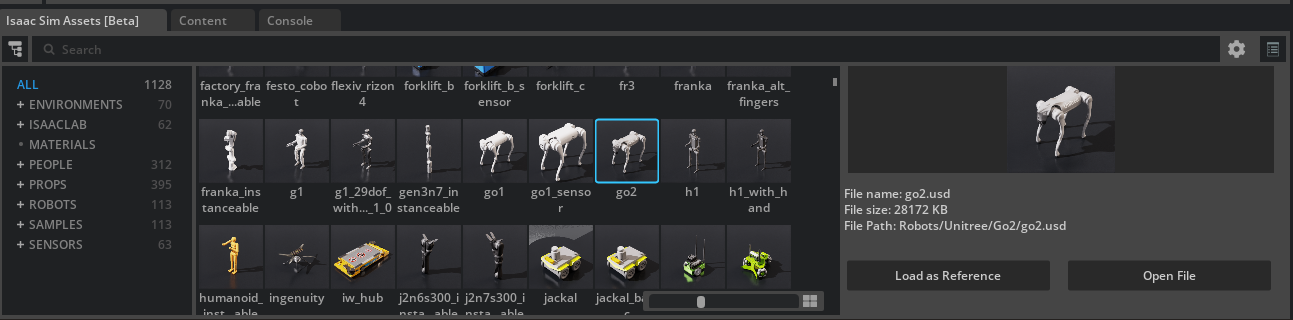
\includegraphics[width=0.75\linewidth]{Zdjęcia/bibliotekaAssets.png}
    \caption{Biblioteka dostępnych robotów Isaac Sim Assets.}
    \label{fig:Assets}
\end{figure}



\begin{figure}[h]
    \centering
    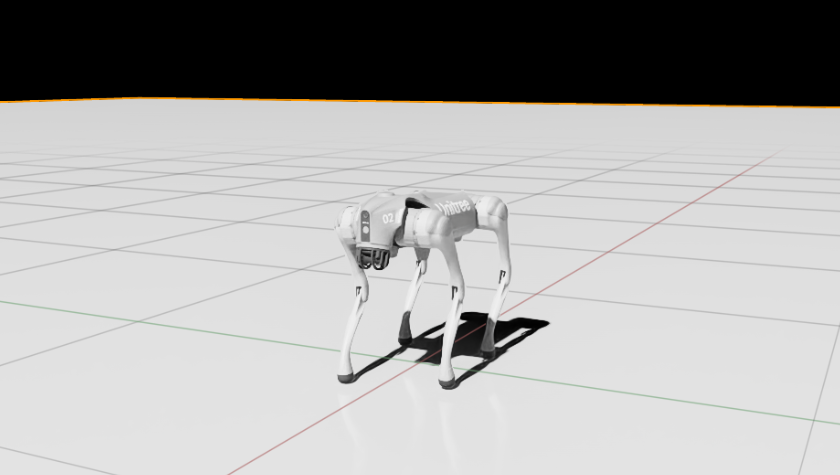
\includegraphics[width=0.75\linewidth]{Zdjęcia/cyfrowyBlizniakUnitryGo2.png}
    \caption{Cyfrowy bliźniak robota Unitree Go2 w środowisku ISAAC SIM.}
    \label{fig:cyfrowyBlizniak}
\end{figure}

\begin{figure}[h]
    \centering
    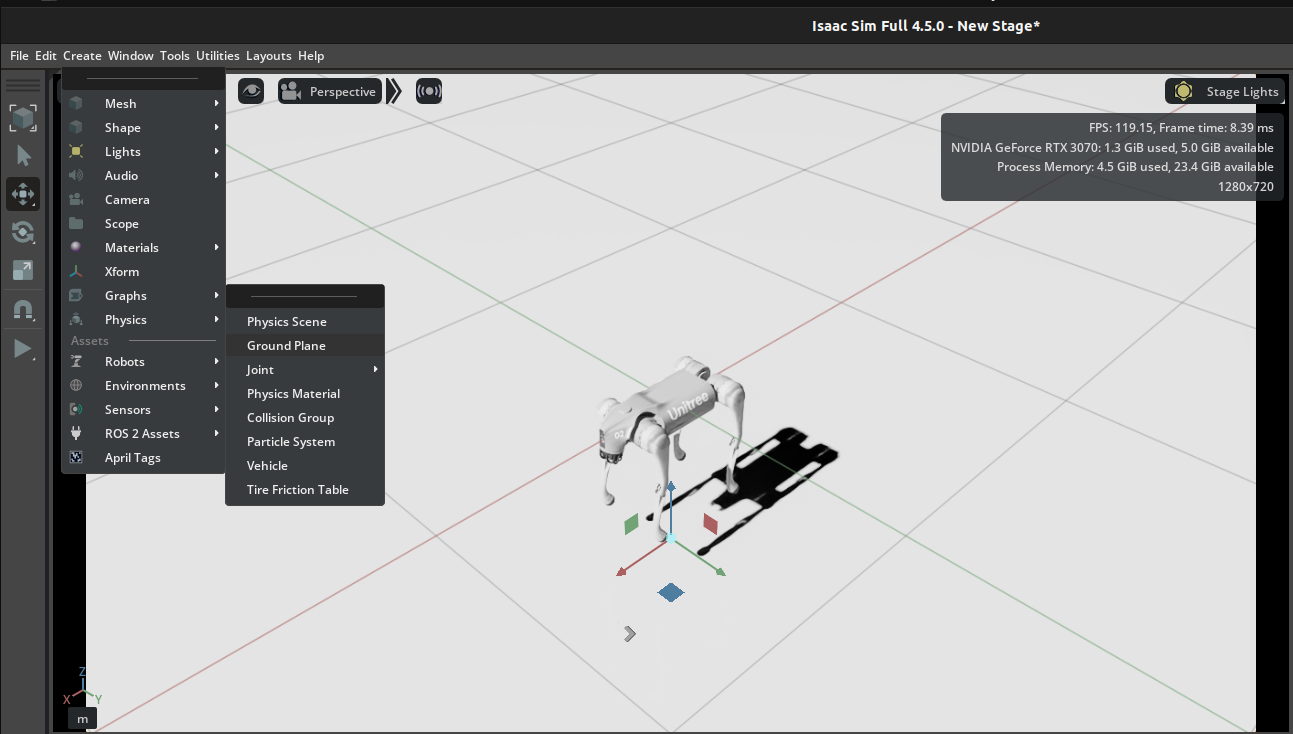
\includegraphics[width=0.9\linewidth]{Zdjęcia/groundPlane.png}
    \caption{Dodanie podłoża w ISSAC SIM.}
    \label{fig:groundPlane}
\end{figure}

\clearpage

\section{Sterowania robotem Unitree Go2 przy pomocy środowiska ROS2}

Wszystkie potrzebne pliki źródłowe do sterowania sterowania robotem znajdują się w linku poniżej.

https://drive.google.com/drive/folders/1fdtBgbXUCxln3wdQgWUAGIBdBf-2Qv9z
\vspace{10pt}

\noindent Żeby możliwe było sterowanie robotem Unitree Go2 przy pomocy środowiska ROS2, wymagane jest dodanie do projektu specjalnego grafu z instrukcjami w formie bloków (Action Graph).Na rysunku \ref{fig:jakDodacAction} pokazane jest jak dodać Action Graph, na rysunku \ref{fig:actionGraph} widoczne są potrzebne do sterowania robotem bloki oraz połączenia między nimi. 

\begin{figure}[h]
    \centering
    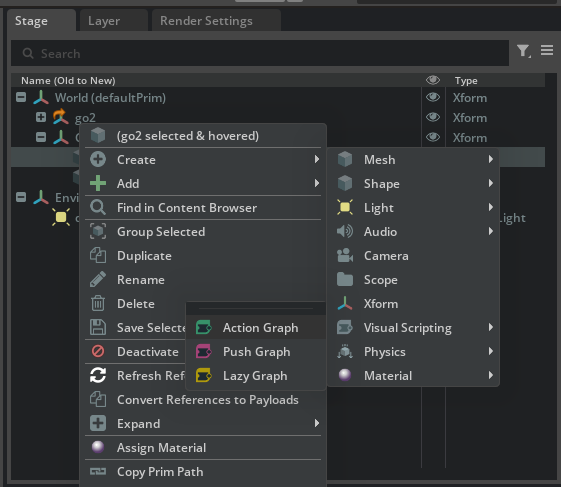
\includegraphics[width=0.7\linewidth]{Zdjęcia/dodanieActionGraph.png}
    \caption{Dodanie Action Graph do cyfrowego bliźniaka Unitree Go2}
    \label{fig:jakDodacAction}
\end{figure}

\clearpage

\begin{figure}[h]
    \centering
    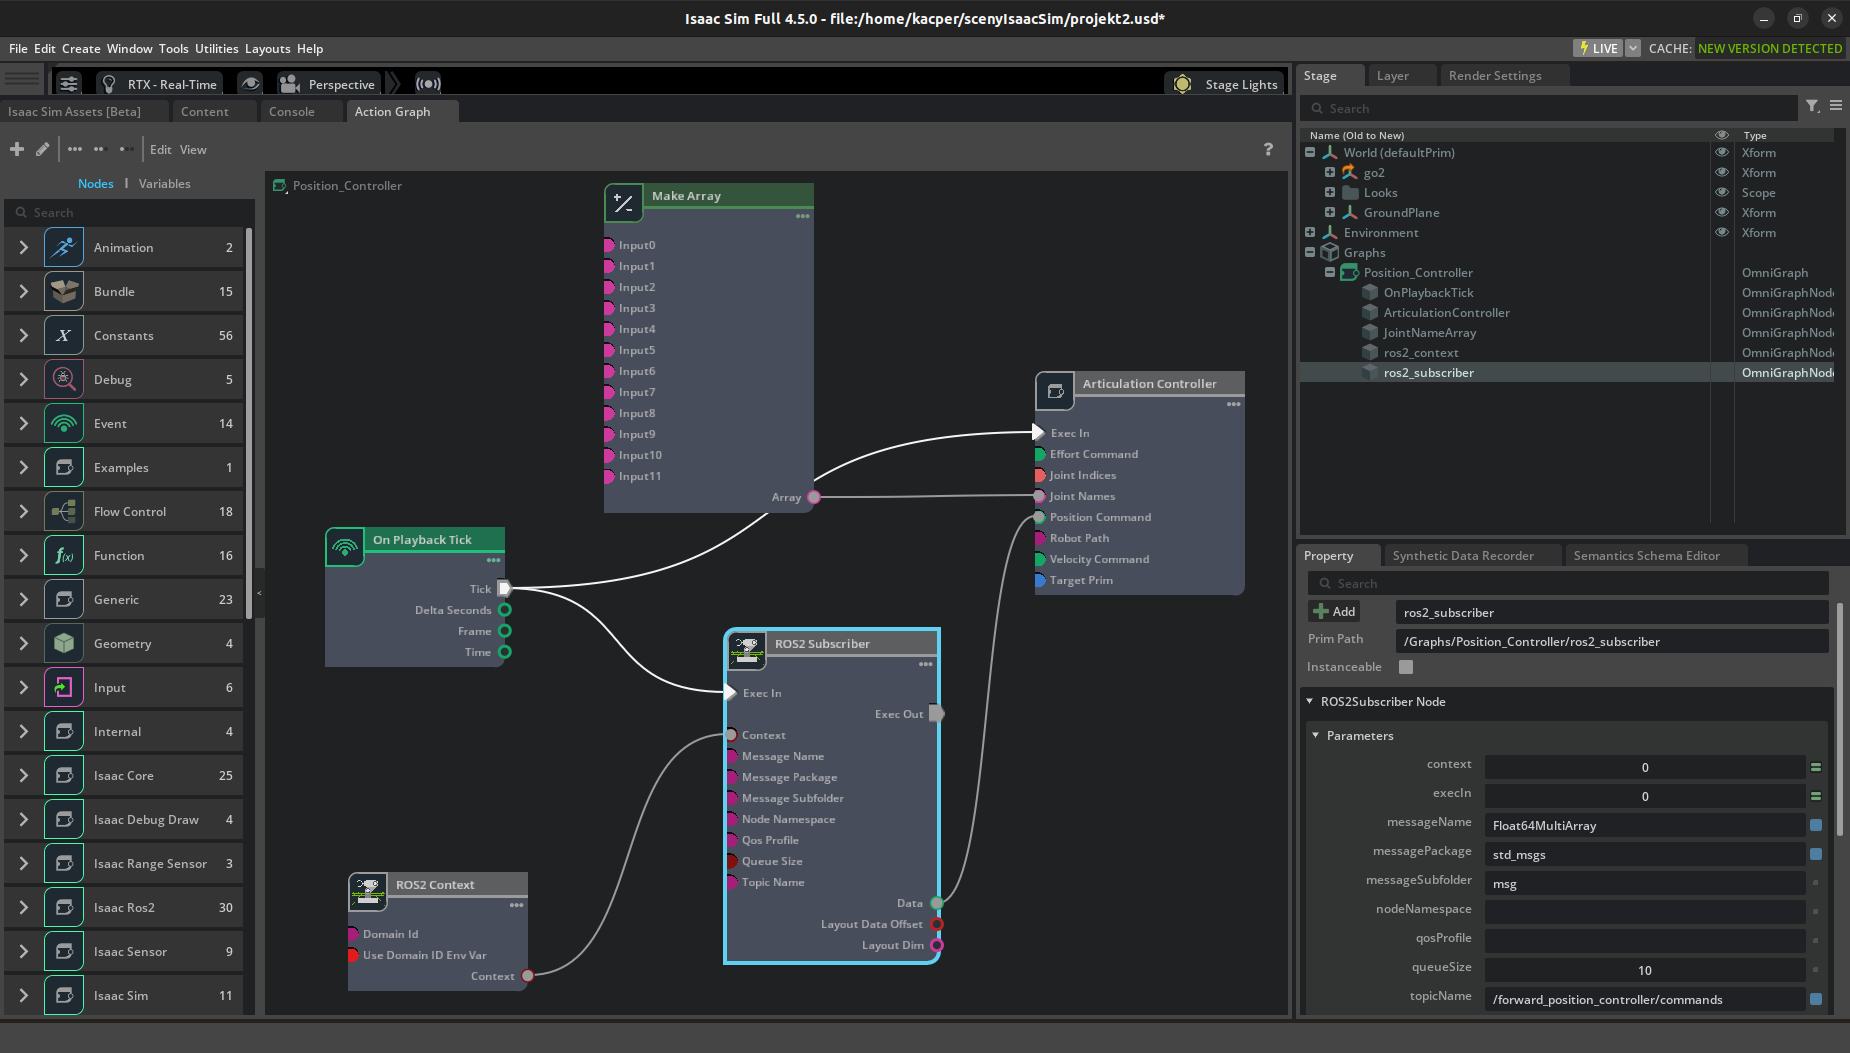
\includegraphics[width=0.75\linewidth]{Zdjęcia/actionGraph.png}
    \caption{Action Graph do nawiązania komunikacji między ROS2 oraz ISAAC SIM.}
    \label{fig:actionGraph}
\end{figure}


\noindent Blok On Playback Tick uruchamia się w każdej klatce symulacji i pozwala na wykonywanie się pozostałych bloków synchronicznie. Blok ROS2 Context inicjalizuję ROS2 w środowisku ISAAC SIM. Articulation Controller służy do przekazywania danych do poszczególnych członów robota. W bloku Make Array należy wstawić poszczególne nazwy członów robota, nazwy te można odczytać z obiektu robota go2. Blok Make Array przekazuje nazwy do bloku Articulation Controller po to żeby wiadomo było jakie człony mają być wysterowane na jaką wartość. Wstawione nazwy członów w bloku Make Array zostały pokazane na rysunku \ref{fig:makeArray} ważne jest żeby kolejność nazw członów była taka sama jak na rysunku, ze względu na fakt, że w takiej kolejności są odbierane z bloku ROS2Subscribe. Kolejność członów w bloku Make Array musi zgadzać się z~ kolejnością członów w kodzie przedstawioną na rysunku \ref{kolejnoscJointow}\\


\begin{figure}[h]
    \centering
    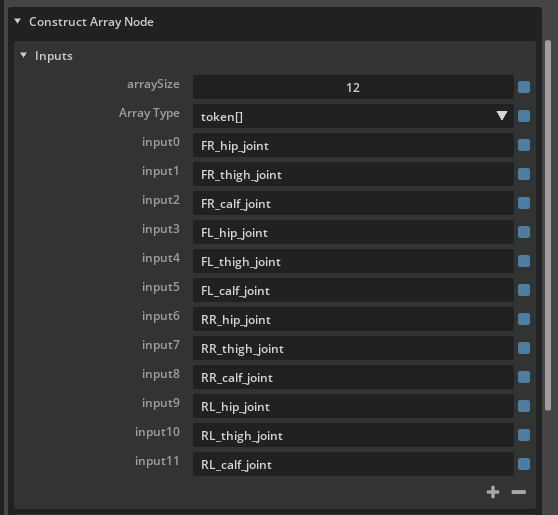
\includegraphics[width=0.5\linewidth]{Zdjęcia/ustawieniaMakeArray.png}
    \caption{Ustawienia bloku Make Array.}
    \label{fig:makeArray}
\end{figure}

\begin{figure}
    \centering
    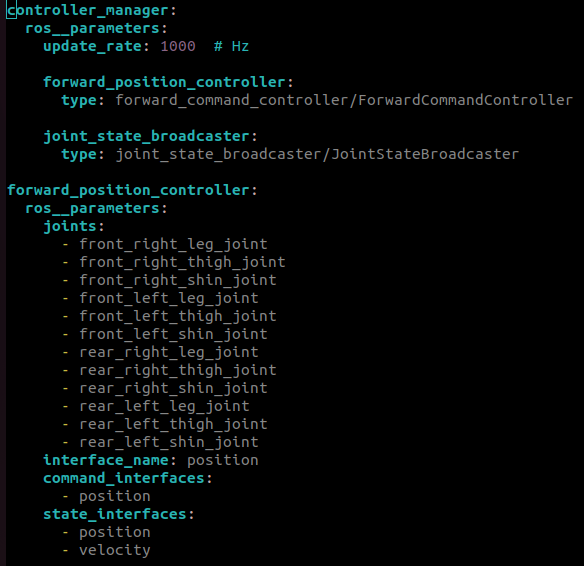
\includegraphics[width=0.5\linewidth]{Zdjęcia/kolejnoscJointow.png}
    \caption{Kolejność członów w kodzie.}
    \label{kolejnoscJointow}
\end{figure}

\noindent Blok ROS2Subscriber służy do otrzymywania danych z programu środowiska ROS2, tak zwanego subskrybowania danych, na rysunku \ref{fig:subscriberROS2} pokazano jak poprawnie skonfigurować blok ROS2Subscriber żeby dane były odpowiednio pobierane. Otrzymane dane są przesyłane do bloku Articulation Controller.\\

\begin{figure}[h]
    \centering
    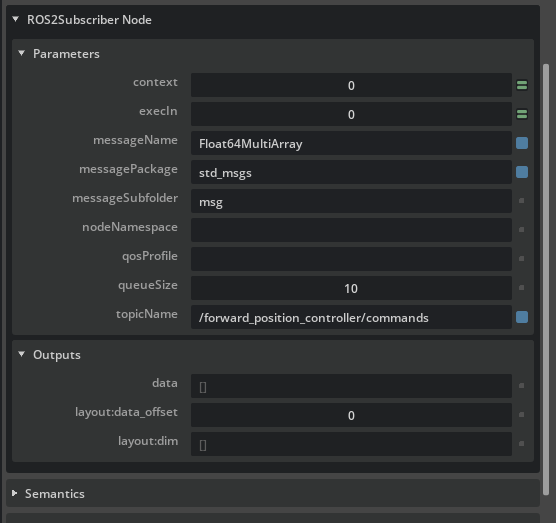
\includegraphics[width=0.5\linewidth]{Zdjęcia/ustawieniaROS2Subsciber.png}
    \caption{Ustawienia bloku ROS2 Subscriber.}
    \label{fig:subscriberROS2}
\end{figure}



\noindent W celu uruchomienia programu sterującego, po wcześniejszym wypakowaniu potrzebnych plików,  należy przejść do folderu $/quadruped\_robot\_ROS2$ i w terminalu wpisać (żeby uruchomić terminal w danym folderze, należy, będąc w aplikacji pliki w danym folderze, wcisnąć prawy przycisk myszy i ‘otwórz w terminalu’):

\noindent $colcon\; build$\\

Następnie w nowym terminalu wpisać:


$source\; quadruped\_robot\_ROS2/install/setup.bash$

$ros2\; launch robot\_control\; robot\_control.launch.py$

\vspace{15px}

 \noindent Po czym przechodzi się do folderu $/qudruped\_robot\_ROS2/UI$ uruchamia się nowy terminal w tym folderze i wpisuje:

$python3\; controller.py$

\clearpage
 
\noindent Na rysunku \ref{fig:pochyleniePrzod} oraz na rysunku \ref{fig:pochylenieTyl} widoczne jest przykładowe sterowanie cyfrowy bliźniakiem robota Unitree Go2. Sterowanie odbywa się przy pomocy okna z kontrolerem widocznego na obu rysunkach, okno ma nazwę controller.



\begin{figure}[h]
    \centering
    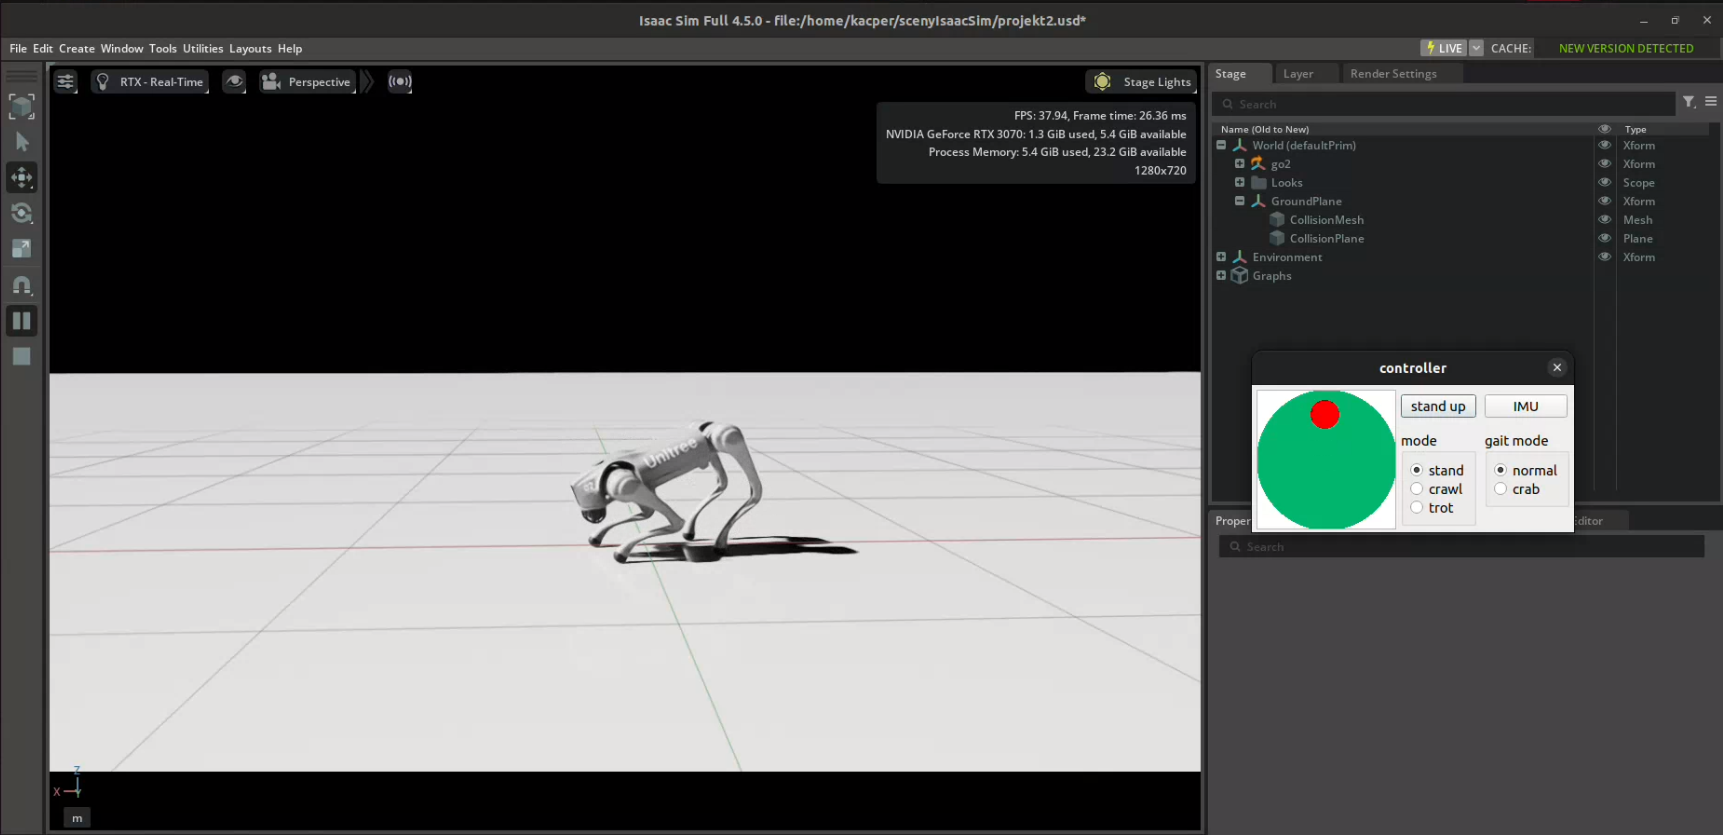
\includegraphics[width=0.8\linewidth]{Zdjęcia/pochyleniePrzod.png}
    \caption{Robot Unitree Go2 pochylający się do przodu.}
    \label{fig:pochyleniePrzod}
\end{figure}

\begin{figure}[h]
    \centering
    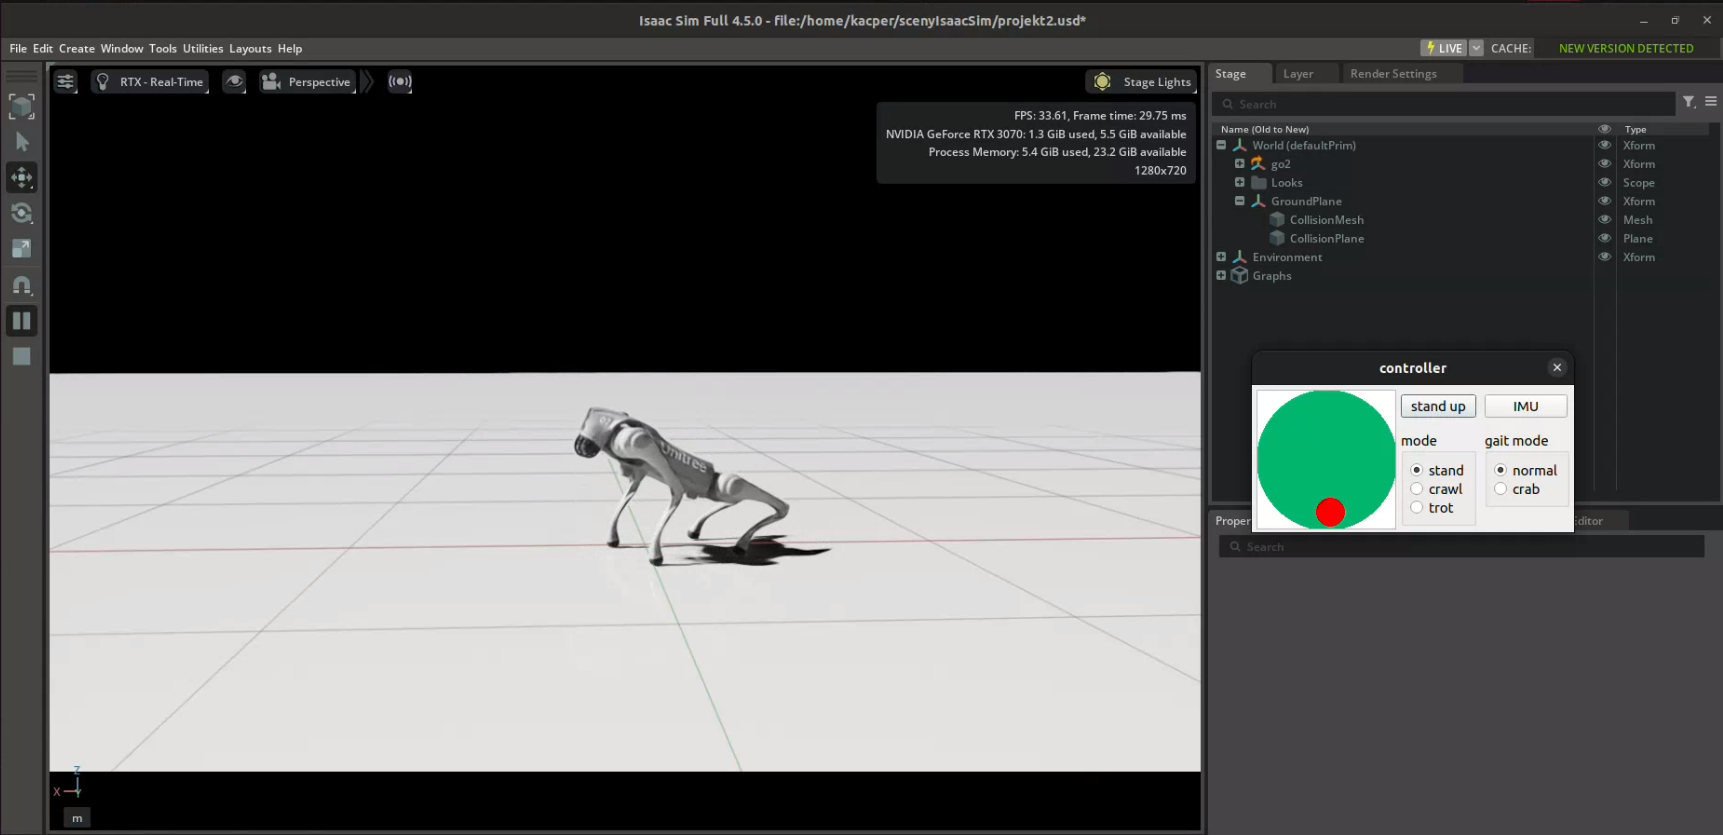
\includegraphics[width=0.8\linewidth]{Zdjęcia/pochylenieTyl.png}
    \caption{Robot Unitree Go2 pochylający się do tyłu.}
    \label{fig:pochylenieTyl}
\end{figure}

Do wykonania tej części projektu korzystaliśmy z poniższego filmu.

\href{https://www.youtube.com/watch?v=L1rpxRm0Q1w&t=581s}{Link do filmu}

\clearpage

\section{Napotkane problemy}
Podczas realizacji projektu związanego z instalacją i konfiguracją środowiska symulacyjnego dla cyfrowego bliźniaka robota Unitree Go2 napotkano szereg problemów technicznych, które wpłynęły na przebieg i czas realizacji poszczególnych etapów. Problemy te dotyczyły zarówno warstwy systemowej (Ubuntu i sterowniki graficzne), jak i aspektów związanych z integracją oprogramowania producenta robota z środowiskiem symulacyjnym IsaacSim i systemem ROS2.\\

\begin{itemize}

  \item \textbf{Problemy ze sterownikami graficznymi} \\
  Jednym z pierwszych istotnych problemów, które wystąpiły już na wczesnym etapie prac, były trudności z poprawnym działaniem środowiska graficznego po instalacji systemu Ubuntu 22.04 oraz komponentów IsaacSim i ROS2. Po zakończeniu instalacji wszystkich wymaganych pakietów oraz pierwszej próbie uruchomienia symulatora pojawiał się błąd związany z działaniem serwera graficznego i interfejsu użytkownika. W efekcie system nie był w stanie prawidłowo załadować środowiska graficznego GNOME lub dochodziło do zawieszeń systemu w trakcie uruchamiania aplikacji korzystających z akceleracji GPU.

  Po analizie logów oraz konsultacji dokumentacji NVIDIA i społeczności użytkowników Ubuntu ustalono, że problem wynikał z niekompatybilnych lub niepełnych wersji sterowników graficznych zainstalowanych domyślnie podczas instalacji systemu. Rozwiązaniem okazało się ręczne pobranie i instalacja najnowszych sterowników NVIDIA bezpośrednio ze strony producenta. Co istotne, proces ten musiał zostać przeprowadzony w trybie tekstowym (bez środowiska graficznego), po wcześniejszym przełączeniu się na tryb wieloużytkownikowy (runlevel 3) i zatrzymaniu serwera X. Po zainstalowaniu sterowników oraz ponownym uruchomieniu systemu, problem z wyświetlaniem grafiki i działaniem Isaac Sim został skutecznie rozwiązany.

  \item \textbf{Problemy po aktualizacji systemu} \\
  Kolejny problem pojawił się w dalszym etapie, po dokonaniu aktualizacji systemu Ubuntu za pomocą standardowego menedżera pakietów. Mimo, że początkowo IsaacSim działał poprawnie, to po zaktualizowaniu systemu oraz ponownym uruchomieniu komputera ponownie wystąpiły błędy graficzne uniemożliwiające uruchomienie środowiska symulacyjnego. System wchodził w tryb awaryjny lub wyświetlał jedynie ekran powitalny bez możliwości zalogowania się do sesji użytkownika.

  Co interesujące, problem ten ustąpił samoistnie po kilku ponownych uruchomieniach systemu oraz zainstalowaniu domyślnych aktualizacji zależności. Nie było konieczności ponownej reinstalacji sterowników graficznych ani środowiska Isaac Sim. Najprawdopodobniej błąd wynikał z tymczasowej niezgodności między wersją jądra systemowego, a zainstalowanym sterownikiem GPU, która została automatycznie rozwiązana po synchronizacji z repozytoriami systemowymi. Problem ten zwrócił jednak uwagę na konieczność ostrożnego zarządzania aktualizacjami w systemach, które wykorzystują dedykowane oprogramowanie zależne od konkretnej wersji jądra i sterowników.

  \item \textbf{Problemy z SDK robota Unitree Go2} \\
  Jednym z kluczowych wyzwań projektu był również brak możliwości wykorzystania oficjalnego SDK dostarczanego przez producenta robota Unitree Go2. Pomimo dostępności dokumentacji oraz kodu źródłowego, SDK okazało się niekompletne i nieprzystosowane do pracy w środowisku symulacyjnym. Pliki nie zawierały pełnych modeli URDF lub SDF, nie istniały odpowiednie definicje do środowisk takich jak IsaacSim, a skrypty sterujące przygotowane były jedynie z myślą o pracy z fizycznym robotem, nie zaś jego cyfrowym odpowiednikiem.

  W celu częściowego obejścia tego problemu podjęto próbę wykorzystania nieoficjalnego repozytorium dostępnego na platformie GitHub, zawierającego zmodyfikowaną wersję SDK oraz częściowo przygotowany model robota. Umożliwiło to podstawową wizualizację i implementację pewnych funkcji, takich jak transmisja danych sensorycznych i wyświetlanie modelu robota w symulatorze. Jednak pomimo tych działań, rozwiązanie to okazało się mało satysfakcjonujące -- ruchy robota były nienaturalne, brakowało płynności animacji, a sterowanie było nieintuicyjne i odbiegało od rzeczywistego zachowania urządzenia.

\end{itemize}

\section{Przykładowe symulacje}

W środowisku ISAAC SIM dostępnych jest wiele przykładowych symulacji do których można uzyskać dostęp wybierając w górnym pasku Window, następnie Examples, a na końcu Robotics Examples, pokazane jest to na rysunku \ref{fig:symulacje}.
W dolnej części programu otwiera się zakładka Robotics Examples, w której znajdują się różnorodne przykłady umożliwiające sterowanie robotami przy pomocy klawiatury. W dalszej części zaprezentowano wybrane przykłady.



\begin{figure}[h]
    \centering
    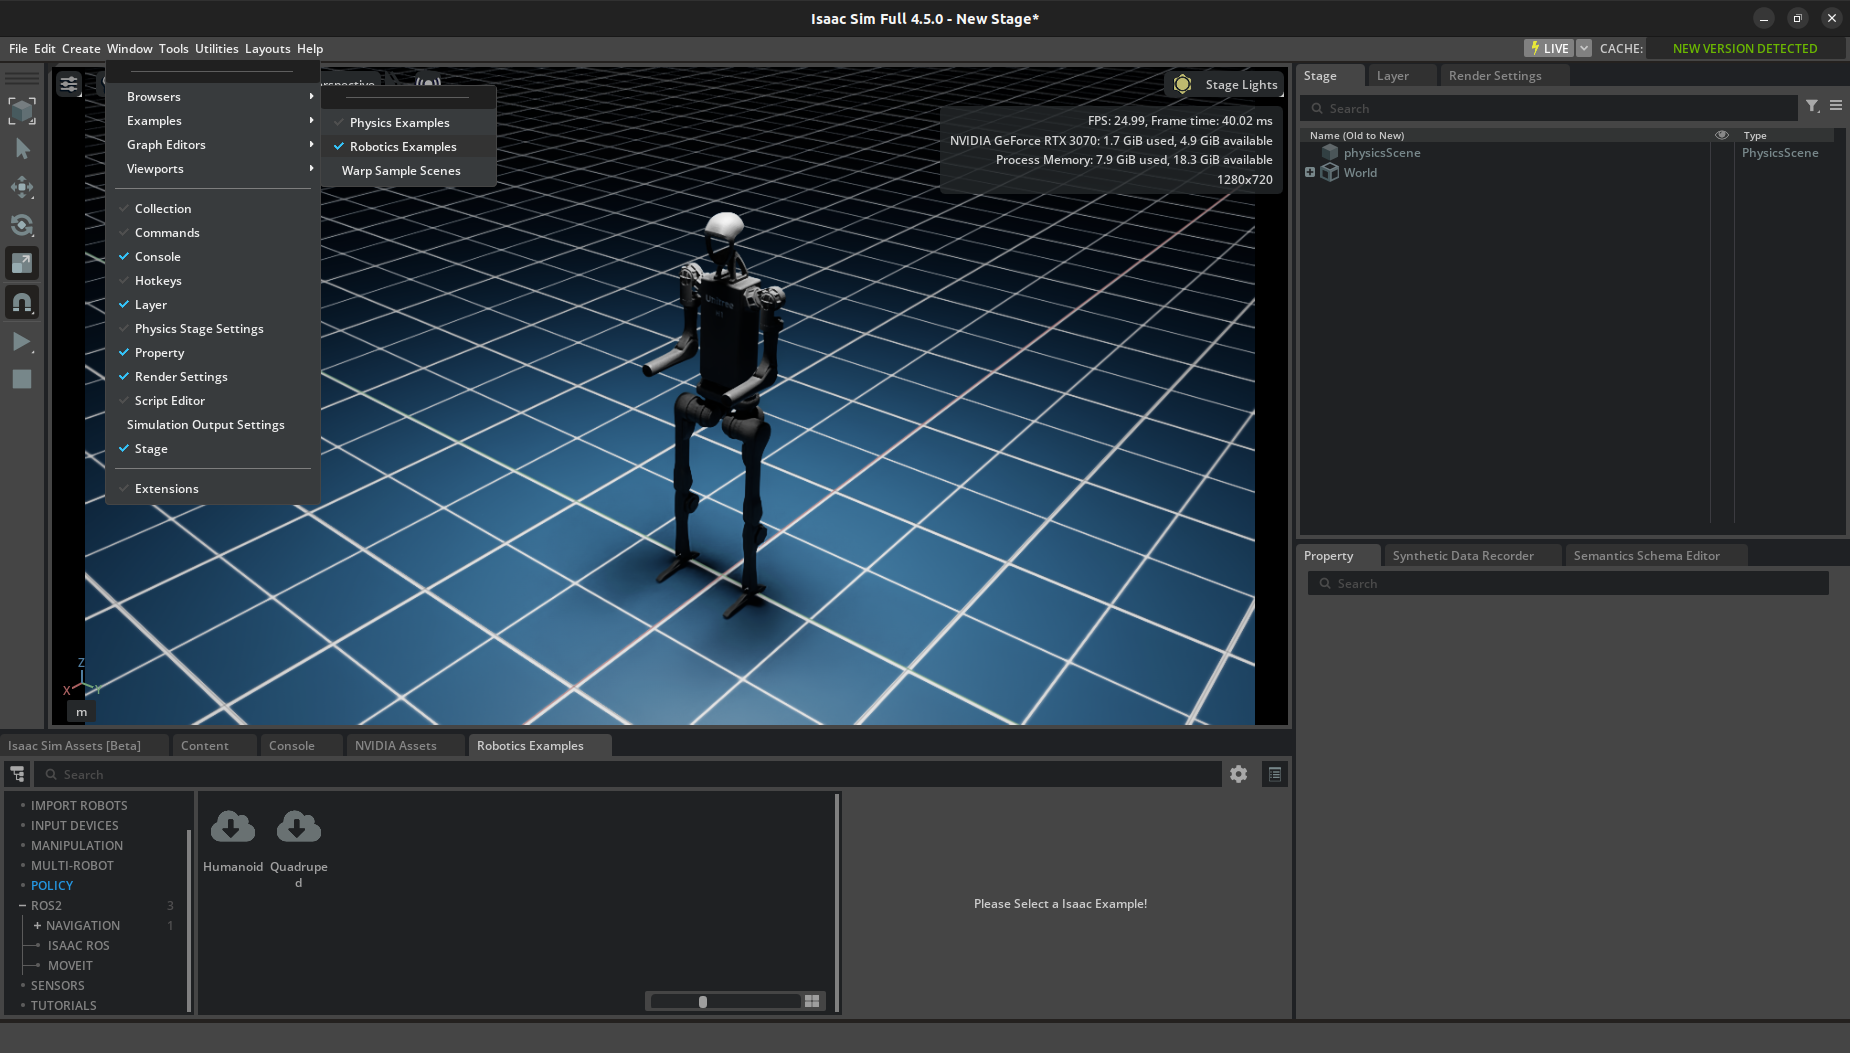
\includegraphics[width=0.8\linewidth]{Zdjęcia/oknoZPrzykladami.png}
    \caption{Okno do dodawania dostępnych w ISAAC SIM przykładowych symulacji.}
    \label{fig:symulacje}
\end{figure}

\newpage

\noindent Na rysunku \ref{fig:bostonDyna} przedstawiony jest widok na cyfrowego bliźniaka firmy Boston Dynamics. W przykładowej symulacji jest możliwe sterowanie nim przy pomocy strzałek i przycisków klawiatury. Sterowanie odbywa się przy pomocy następujących klawiszy: \\ 

\texttt{Klawisz  Działanie}

\texttt{Strzałka w górę/numpad 8  Idź do przodu}

\texttt{Strzałka w dół/numpad 2  Idź do tyłu}

\texttt{Lewa strzałka/numpad 4  Idź w lewo}

\texttt{Prawa strzałka/numpad 6  Idź w prawo}

\texttt{N/numpad 7  Kręć się przeciwnie do ruchu wskazówek zegara}

\texttt{M/numpad 9 Kręć się zgodnie z ruchem wskazówek zegara}\\

\noindent Rysunek \ref{fig:humanoid} pokazuje humanoidalnego robota firmy Unitree, którym również możliwe jest sterowanie w~ dostępnej przykładowej symulacji. Sterowanie odbywa się przy pomocy: \\

\texttt{Klawisz  Działanie}

\texttt{Strzałka w górę/numpad 8  Idź do przodu}

\texttt{Strzałka w lewo/numpad 4 Kręć się przeciwnie do ruchu wskazówek zegara}

\texttt{Strzałka w prawo/numpad 6 Kręć się zgodnie z ruchem wskazówek zegara}

\begin{figure}[h]
    \centering
    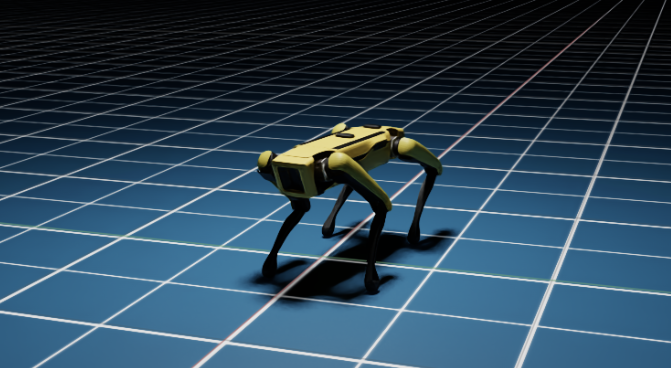
\includegraphics[width=0.8\linewidth]{Zdjęcia/przykladBoston.png}
    \caption{Przykład z ISAAC SIM z robotem Boston Dynamics.}
    \label{fig:bostonDyna}
\end{figure}

\begin{figure}[h]
    \centering
    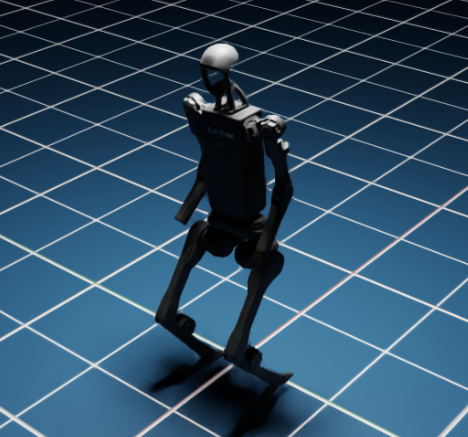
\includegraphics[width=0.5\linewidth]{Zdjęcia/przykladHumanoid.png}
    \caption{Przykład z ISAAC SIM z robotem humanoidalny.}
    \label{fig:humanoid}
\end{figure}

W środowisku ISAAC SIM dostępny jest też przykład z manipulatorem układającym kolejne dostarczane przez ruchomy taśmociąg palety. Okno z widoku tej przykładowej symulacji jest pokazane na rysunku \ref{fig:palety}.

\begin{figure}[h]
    \centering
    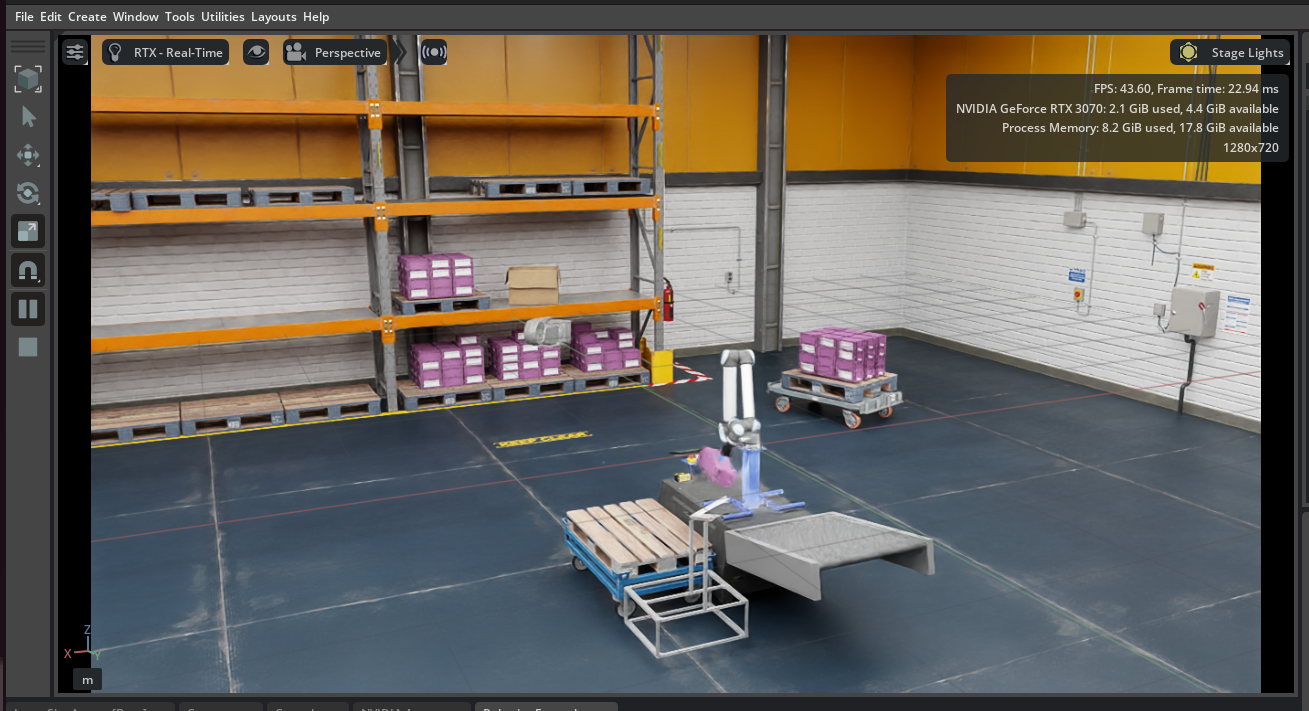
\includegraphics[width=0.7\linewidth]{Zdjęcia/przykladowaPaletyzacja.png}
    \caption{Przykład z ISAAC SIM z manipulatorem i paletami.}
    \label{fig:palety}
\end{figure}

Na rysunku \ref{IMU} przedstawiony jest przykład z czujnikiem IMU, gdzie możliwe jest poruszanie obiektem i~ obserwowanie zmian wartości zwracanych przez czujnik IMU. Rysunek \ref{ruchIMU} pokazuje, jak poruszanie obiektem wpływa na zmianę wartości mierzonych przez czujnik IMU. Sterowanie odbywa się poprzez jednoczesne wciśnięcie shift oraz lewego przycisku myszy na obiekcie pozwala to na poruszanie nim przez ruchy myszki.

\begin{figure}[h]
    \centering
    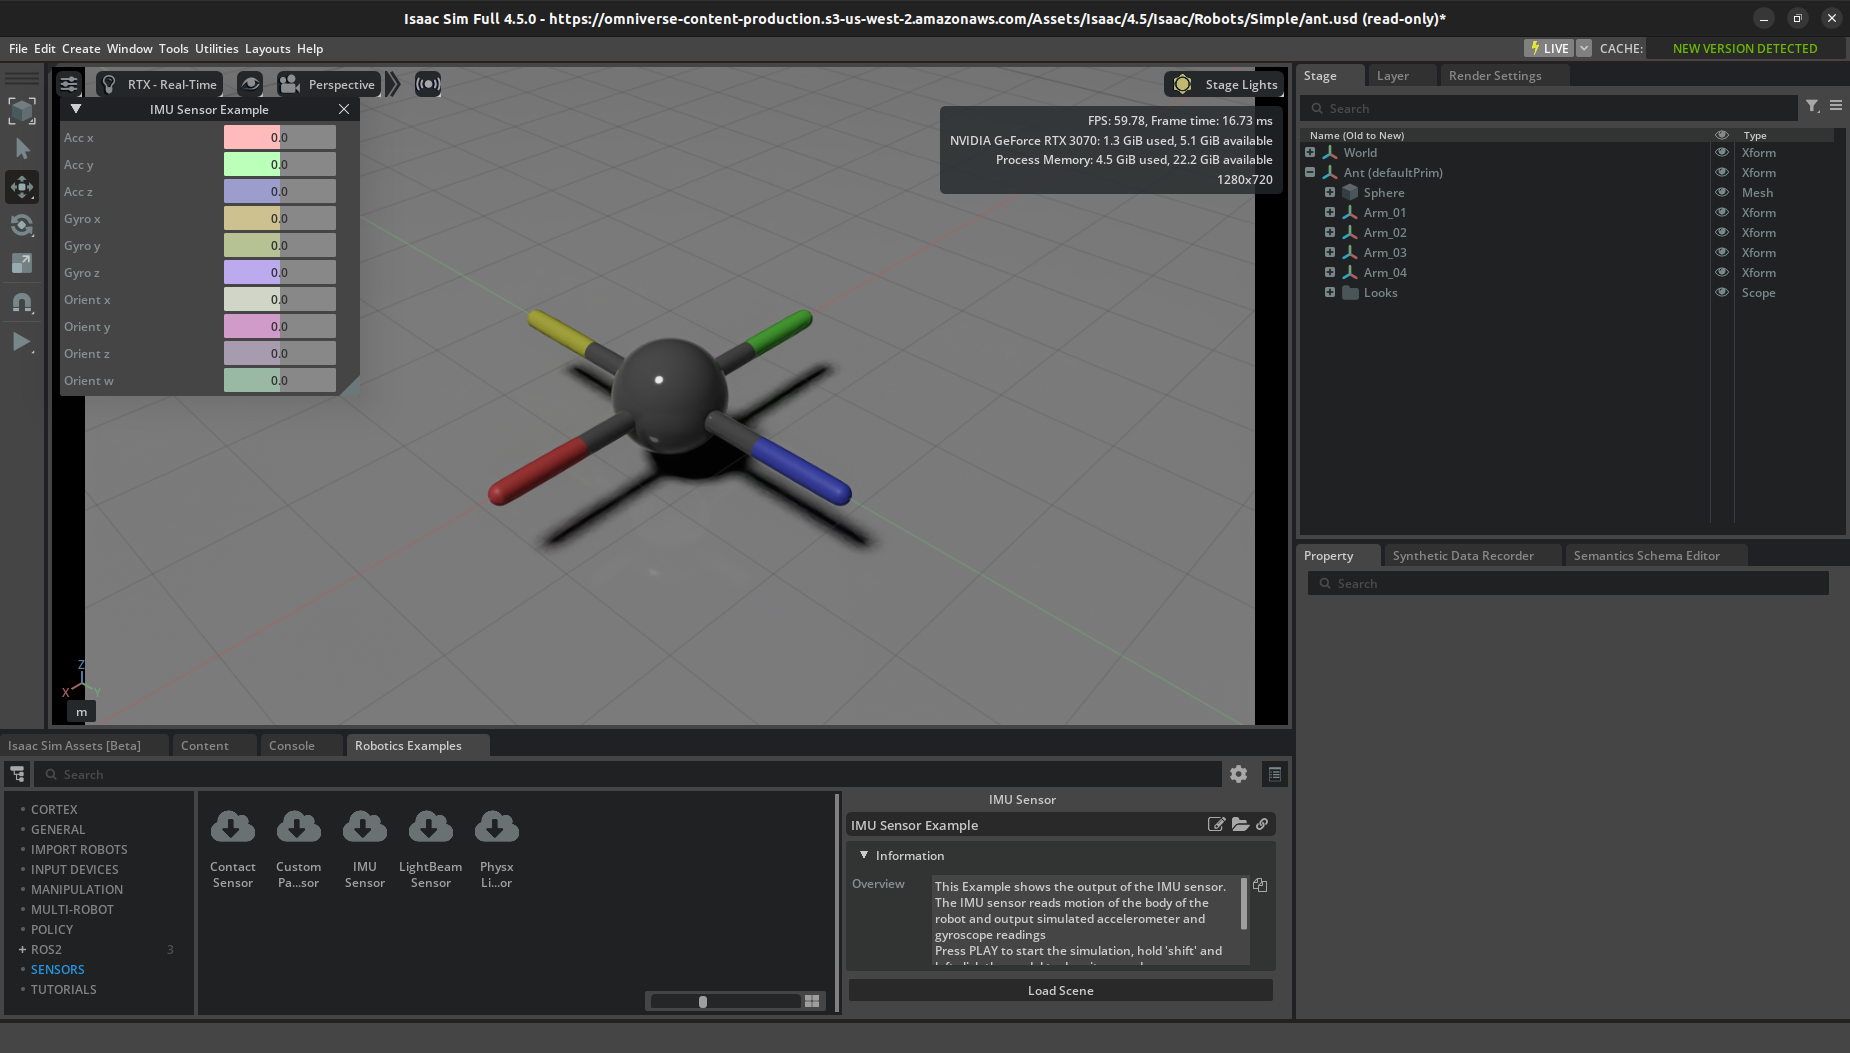
\includegraphics[width=0.7\linewidth]{Zdjęcia/czujnikIMU.png}
    \caption{Przykład z ISAAC SIM z czujnikiem IMU.}
    \label{IMU}
\end{figure}

\begin{figure}
    \centering
    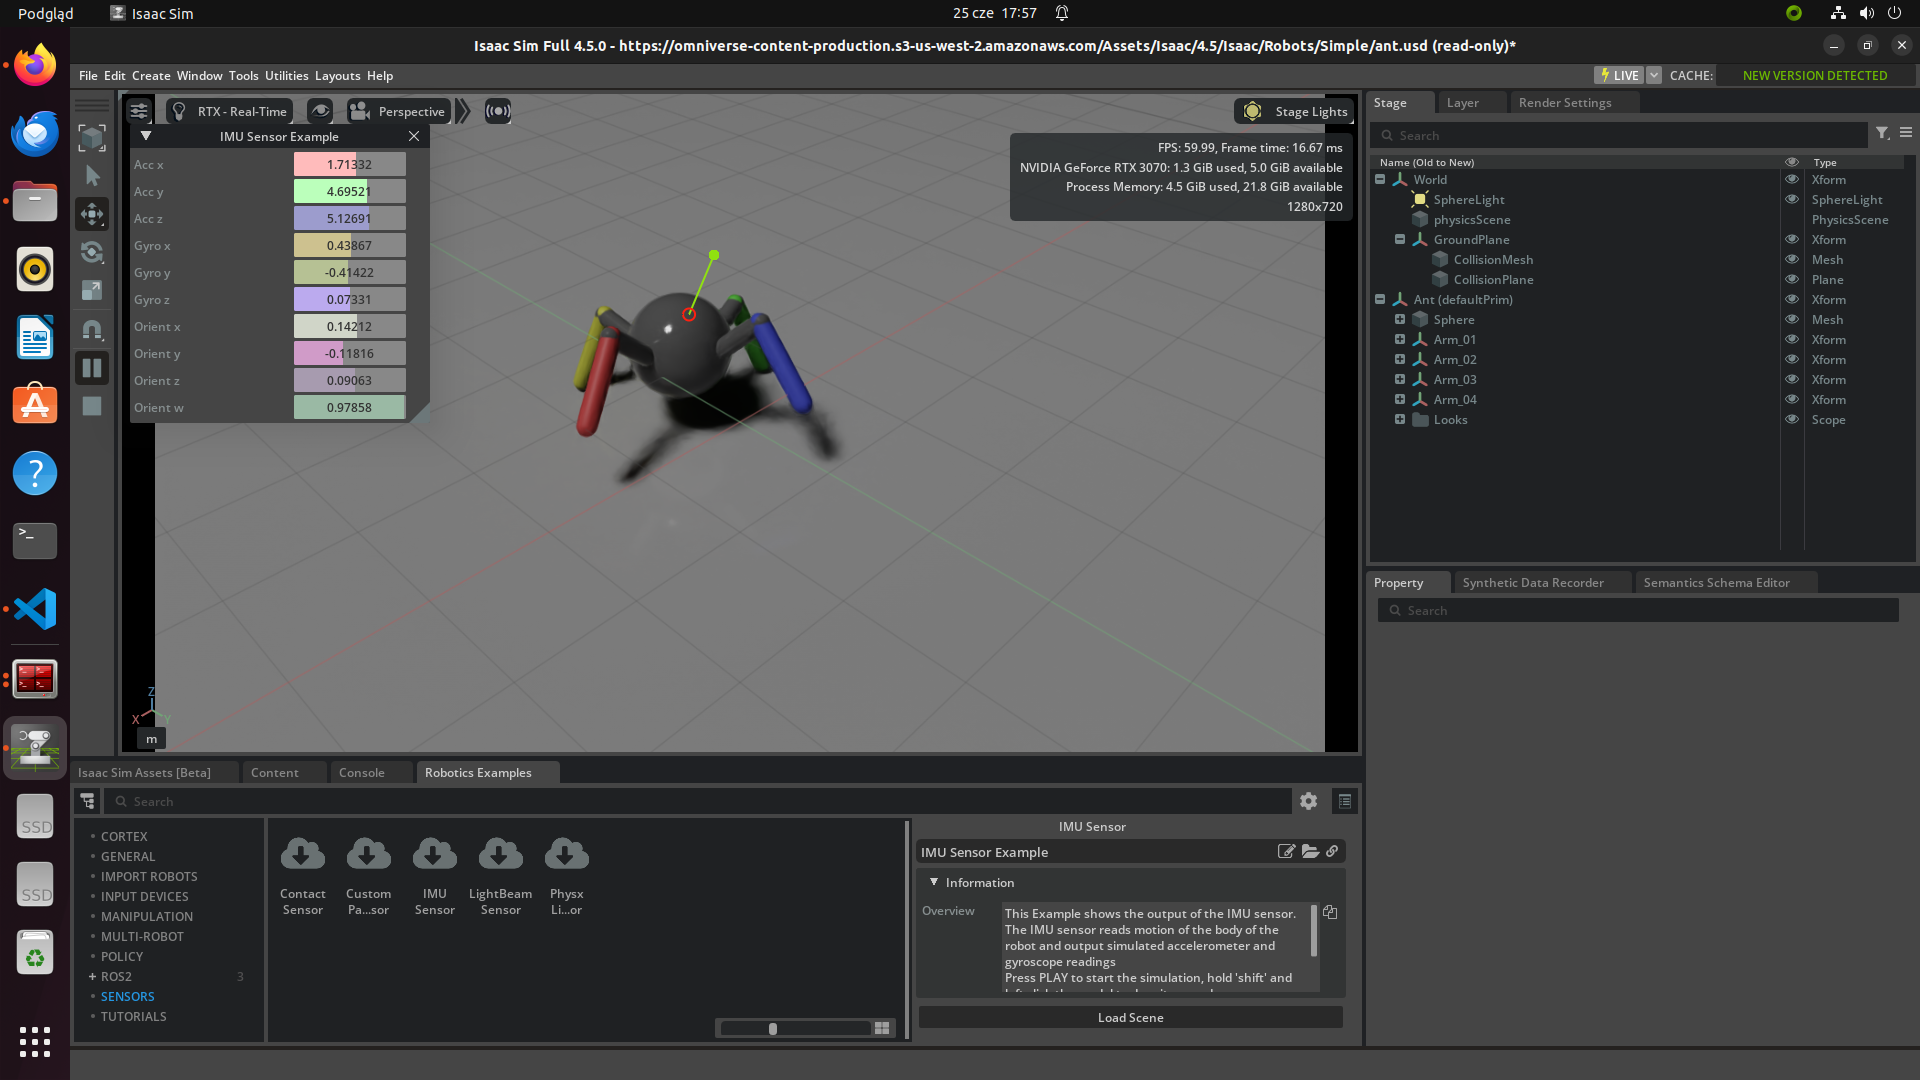
\includegraphics[width=0.7\linewidth]{Zdjęcia/poruszanieIMU.png}
    \caption{Przykład z ISAAC SIM z czujnikiem IMU i poruszaniem obiektem.}
    \label{ruchIMU}
\end{figure}

\clearpage

\section{Podsumowanie osiągniętych celów projektu}

W trakcie wykonywania projektu udało się wykonać wszystkie narzucone odgórnie cele narzucone w nim. Czyli:
\begin{itemize}
    \item Zainstalowano środowisko ISAAC SIM
    \item Skonfigurowano środowisko tak, żeby możliwa była jego komunikacja z ROS2
    \item W symulacji został przygotowany cyfrowy bliźniak robota Unitree Go2
    \item Nawiązano połączenie między środowiskiem ISAAC SIM oraz ROS2
    \item Cyfrowy bliźniak robota Unitree Go2 był sterowany w środowisku ISAAC SIM przy użyciu ROS2
    \item Przeprowadzono sterowanie robotem kołowym z użyciem ROS2 w symulacji ISAAC SIM
    \item Testowano przykładowe symulacje znajdujące się w ISAAC SIM, między innymi sterowanie robotem humanoidalnym i robotem czworonożnym przy pomocy klawiatury oraz przykład symulacji z ramieniem robota ustawiającym palety 
    
\end{itemize}

\section{Propozycje dalszego rozwoju}

Do propozycji dalszego rozwoju należą:
\begin{itemize}
    \item Poprawa algorytmu sterującego cyforwym bliźniakiem robota Unitree Go2 lub napisanie całego algorytmu od nowa
    \item Sterowanie cyfrowym bliźniakiem innego robota przy pomocy ROS2
    \item Stworzenie własnego modelu URDF robota i sterowanie nim w środowisku ISAAC SIM
    \item Dodanie czujników do cyfrowego bliźniaka robota Unitree Go2
\end{itemize}

\section{Dokumentacja}

\begin{itemize}
  \item \textbf{Isaac Sim}
  \begin{itemize}
    \item \url{https://docs.isaacsim.omniverse.nvidia.com/latest/reference_material/reference_glossary.html}
    \item \url{https://docs.isaacsim.omniverse.nvidia.com/latest/index.html}
  \end{itemize}

  \item \textbf{Unitree Go2}
  \begin{itemize}
    \item \url{https://unitree.arcsecondrobo.net/detail?id=28}
    \item \url{https://support.unitree.com/home/en/developer/Software_Interface_Services}
    \item \url{https://www.unitree.com/opensource}
    \item \url{https://github.com/wing-kit/unitree_go2_ros2}
    \item \url{https://github.com/unitreerobotics}
  \end{itemize}

  \item \textbf{ROS~2}
  \begin{itemize}
    \item \url{https://docs.ros.org/en/foxy/index.html}
    \item \url{https://docs.ros.org/en/humble/Releases.html}
  \end{itemize}

  \item \textbf{Materiały wideo}
  \begin{itemize}
    \item \url{https://www.youtube.com/watch?v=3cWQsvpwvQU}
    \item \url{https://www.youtube.com/watch?v=OcqzPEJWnms}
    \item \url{https://www.youtube.com/watch?v=L1rpxRm0Q1w}
    \item \url{https://www.youtube.com/watch?v=ithYYtUduMQ}
    \item \url{https://www.youtube.com/watch?v=Wnd5IUNbXnI}
    \item \url{https://www.youtube.com/watch?v=YSedTUxI0wc}
    \item \url{https://www.youtube.com/watch?v=Tb5Pp2fSwSw}
    \item \url{https://www.youtube.com/watch?v=tTCbdul7xsc}
    \item \url{https://www.youtube.com/watch?v=1f_5smH_AYM}
    \item \url{https://www.youtube.com/watch?v=L1rpxRm0Q1w&t=581s}
  \end{itemize}
\end{itemize}


\end{document}
